\documentclass[a4paper, oneside]{article}
\usepackage{castle_of_magic}
\usepackage[margin=0.125in]{geometry}
\usepackage[skip=0pt]{parskip}
\usepackage{enumitem}
\usepackage{setspace}

\begin{document}
\setmainfont[Scale=1.0]{TeX Gyre Chorus}\phantom{a}%\setmainfont[Scale=3.0]{TeX Gyre Chorus}
\begin{center}
\begin{tikzpicture}[x=1in, y=1in]
\pic[scale=1.5, transform shape] () at (0,0) {player_aid_scoring={eaglered}};
\node at (0,0) {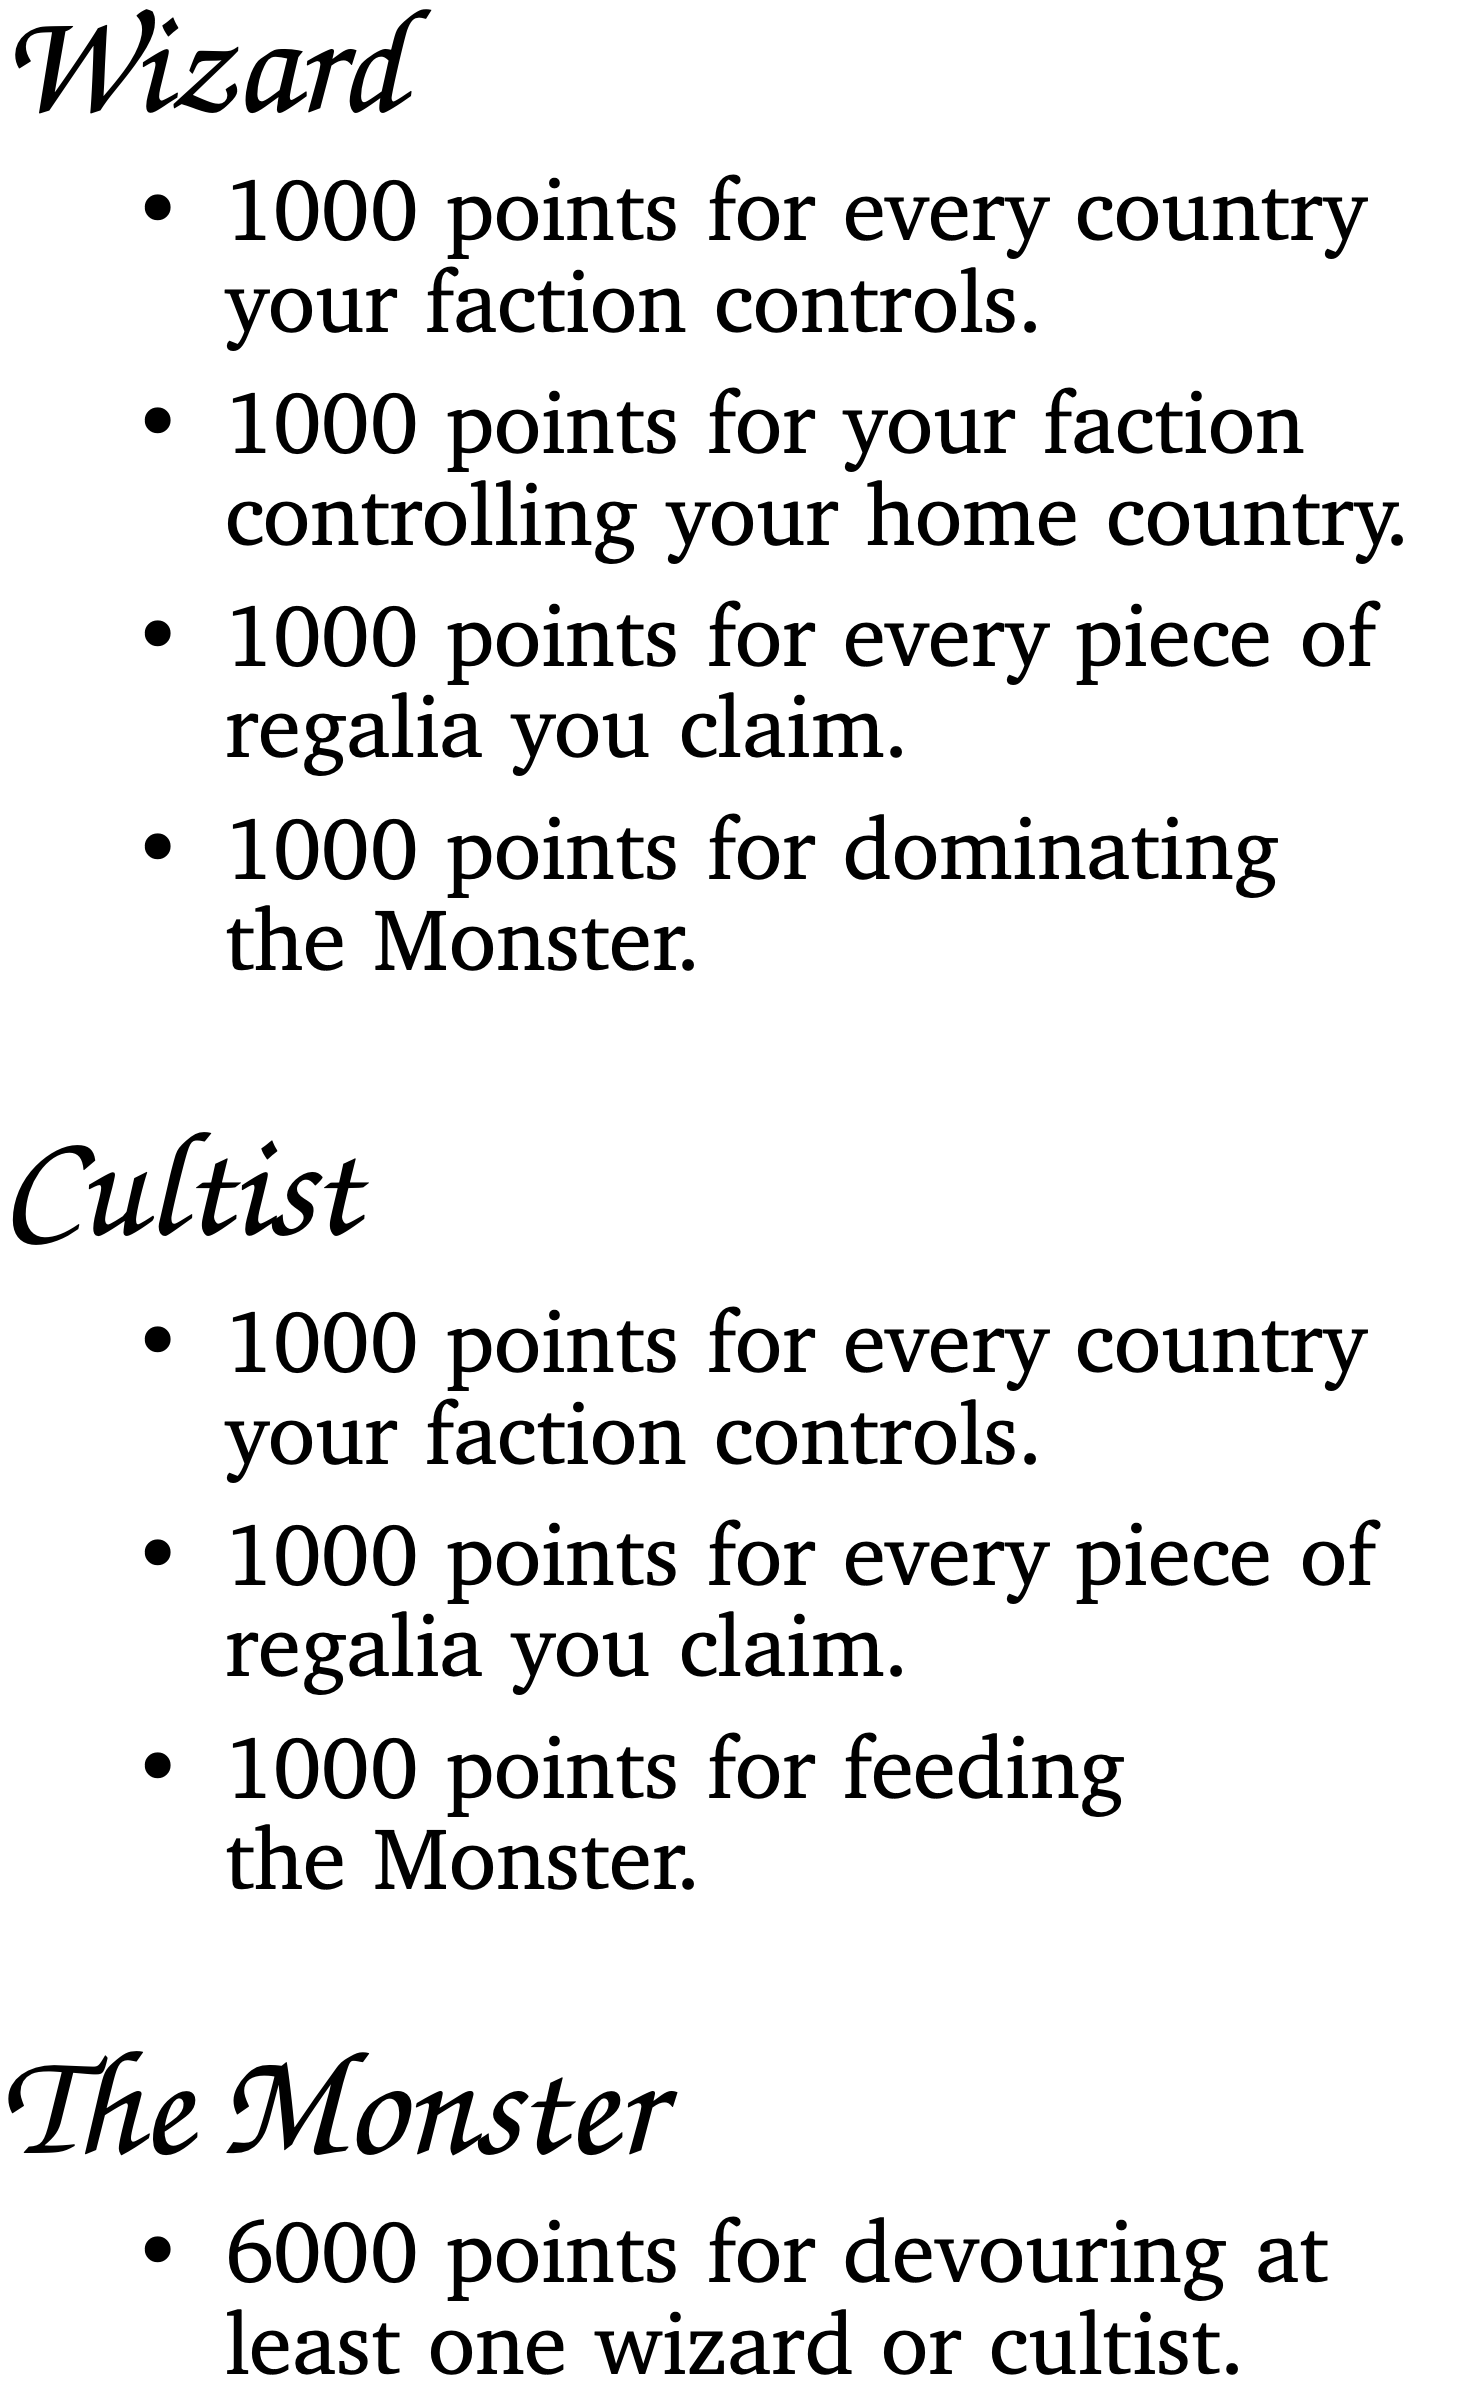
\includegraphics[scale=0.12]{player_aid_scoring_text.png}};
\pic[scale=1.5, transform shape] () at (0,0) {cutguide={black}};
\pic[scale=1.5, transform shape] () at (1.5\horizdist,0) {player_aid_scoring={Orange}};
\node at (1.5\horizdist,0) {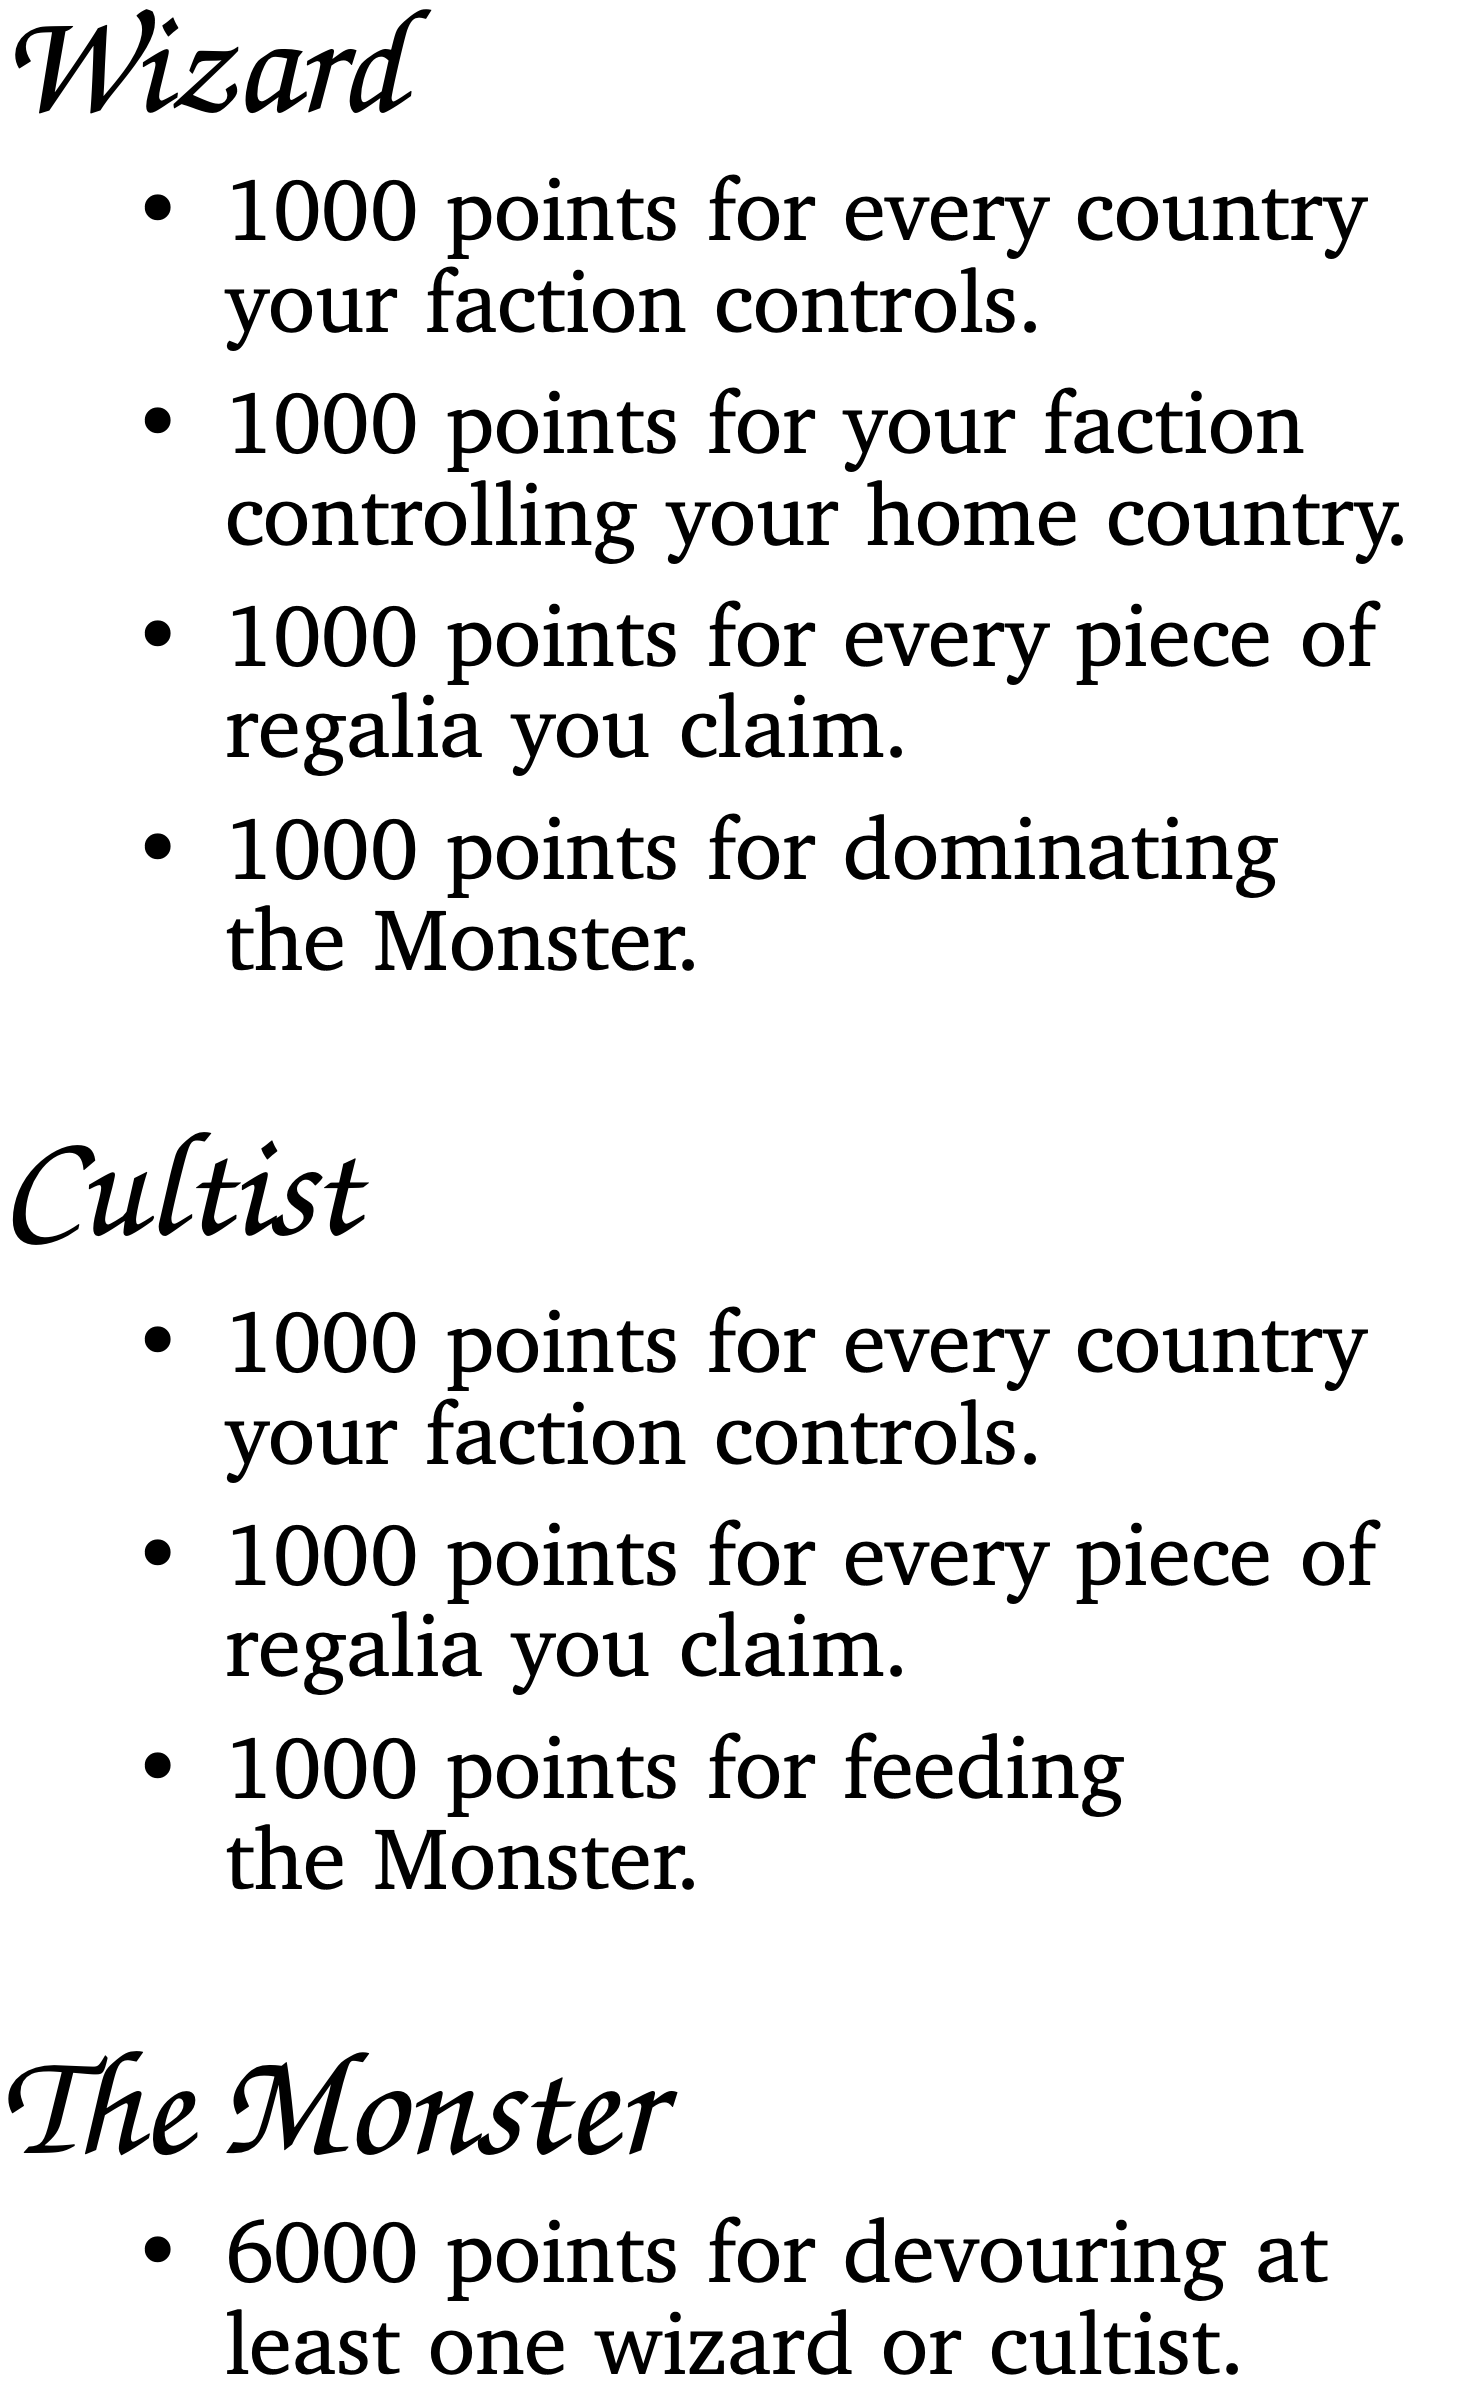
\includegraphics[scale=0.12]{player_aid_scoring_text.png}};
\pic[scale=1.5, transform shape] () at (1.5\horizdist,0) {cutguide={black}};

\pic[scale=1.5, transform shape] () at (0,-1.5\vertdist) {player_aid_scoring={dragongreen}};
\node at (0,-1.5\vertdist) {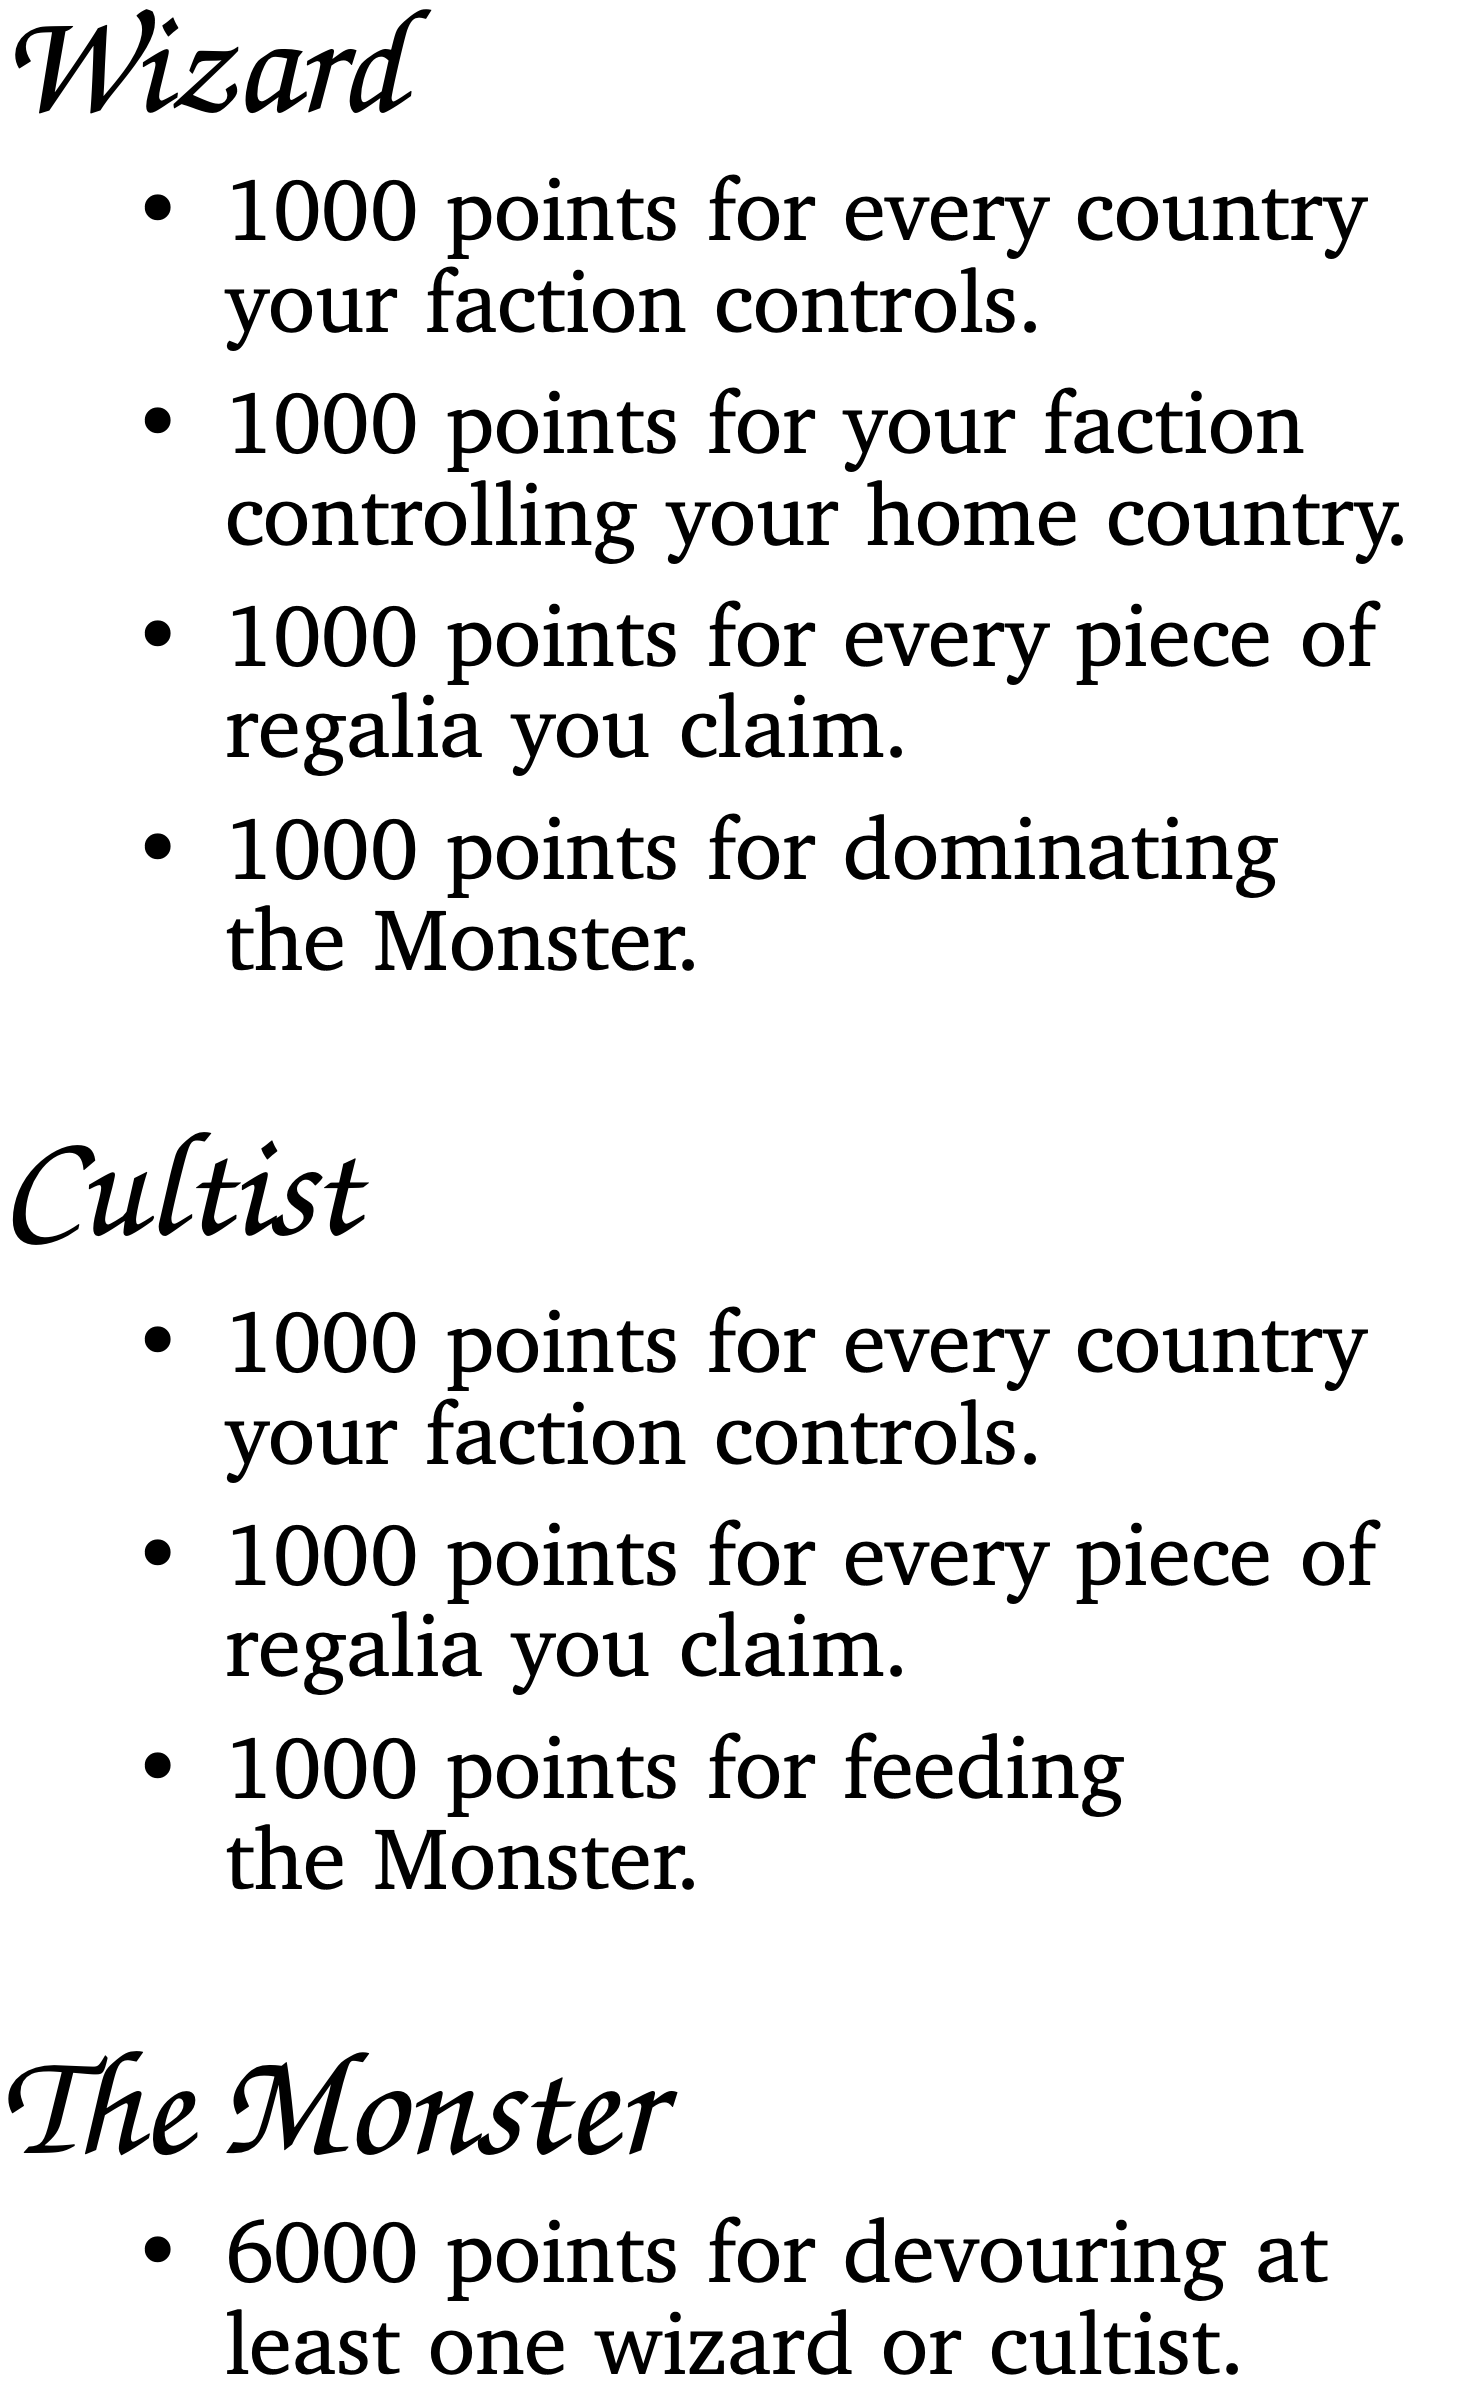
\includegraphics[scale=0.12]{player_aid_scoring_text.png}};
\pic[scale=1.5, transform shape] () at (0,-1.5\vertdist) {cutguide={black}};
\pic[scale=1.5, transform shape] () at (1.5\horizdist,-1.5\vertdist) {player_aid_scoring={wolfblue}};
\node at (1.5\horizdist,-1.5\vertdist) {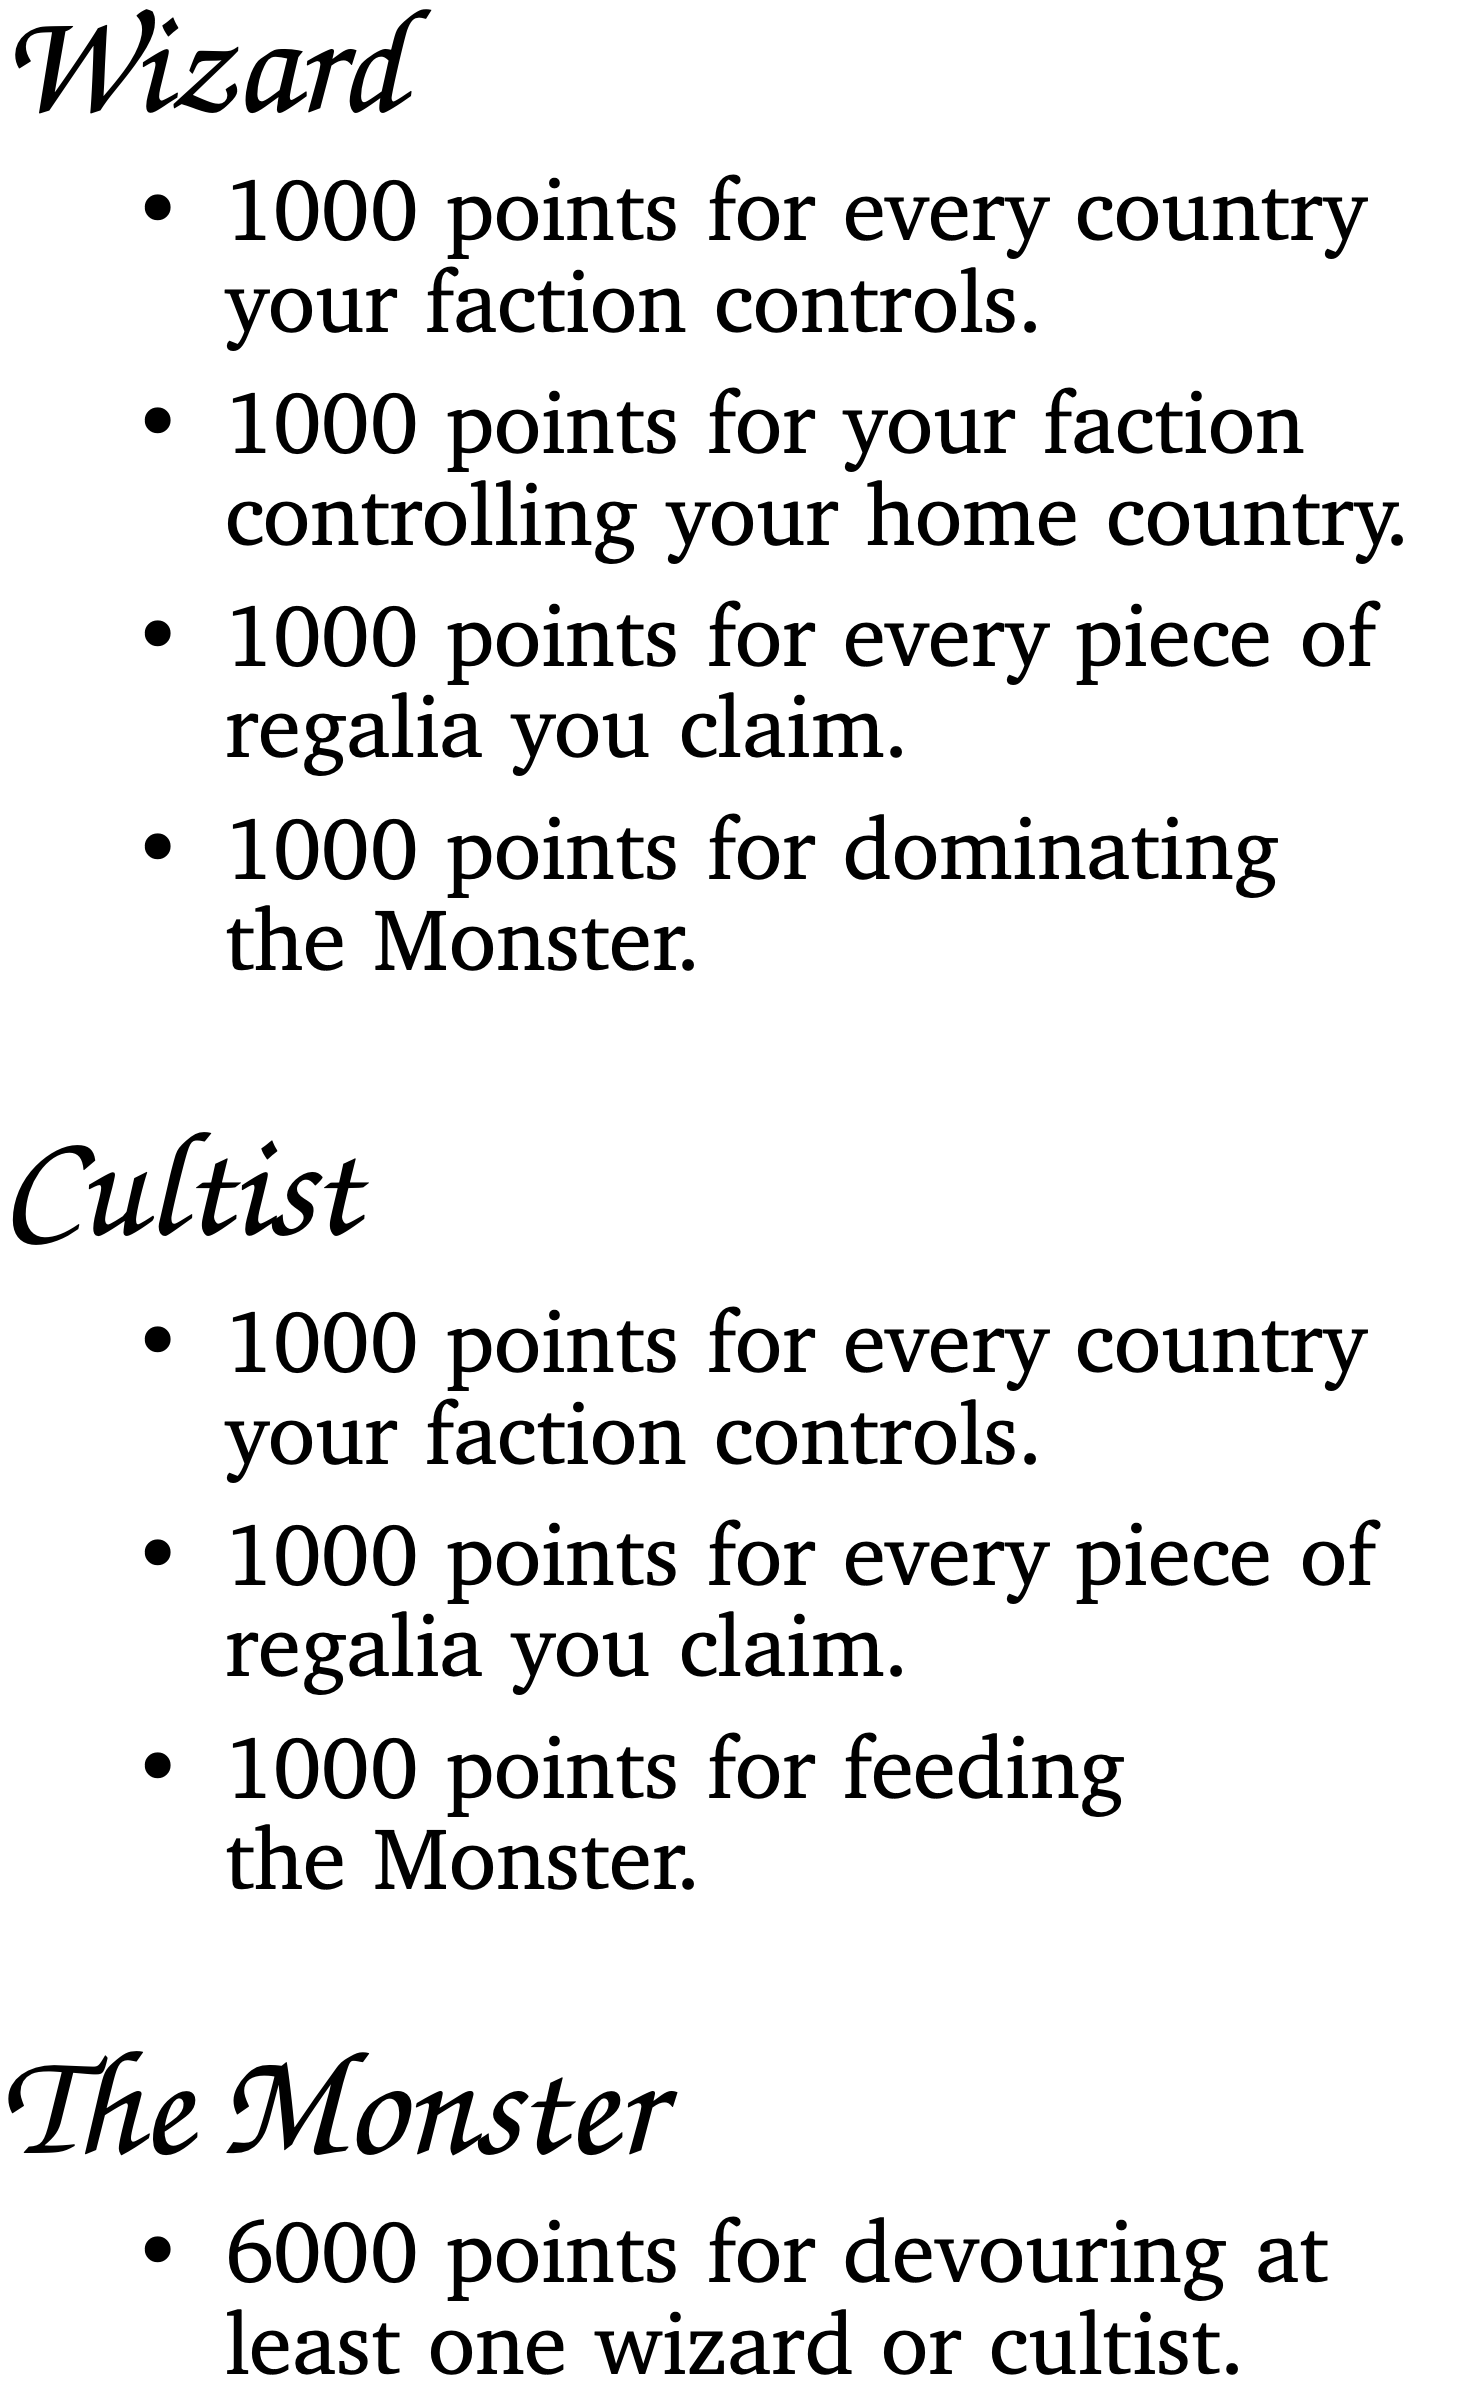
\includegraphics[scale=0.12]{player_aid_scoring_text.png}};
\pic[scale=1.5, transform shape] () at (1.5\horizdist,-1.5\vertdist) {cutguide={black}};
\end{tikzpicture}	
\end{center}
\newpage
\setmainfont[Scale=1.0]{TeX Gyre Chorus}\phantom{a}%\setmainfont[Scale=3.0]{TeX Gyre Chorus}
\begin{center}
\begin{tikzpicture}[x=1in, y=1in, transform shape]
%\pic () at (0,0) {player_aid_turns={kidagold}};
%\pic () at (0,0) {cutguide={kidagold}};
\pic[scale=1.5, transform shape] () at (0, 0) {player_aid_turns={Orange}};
\node at (0,0) {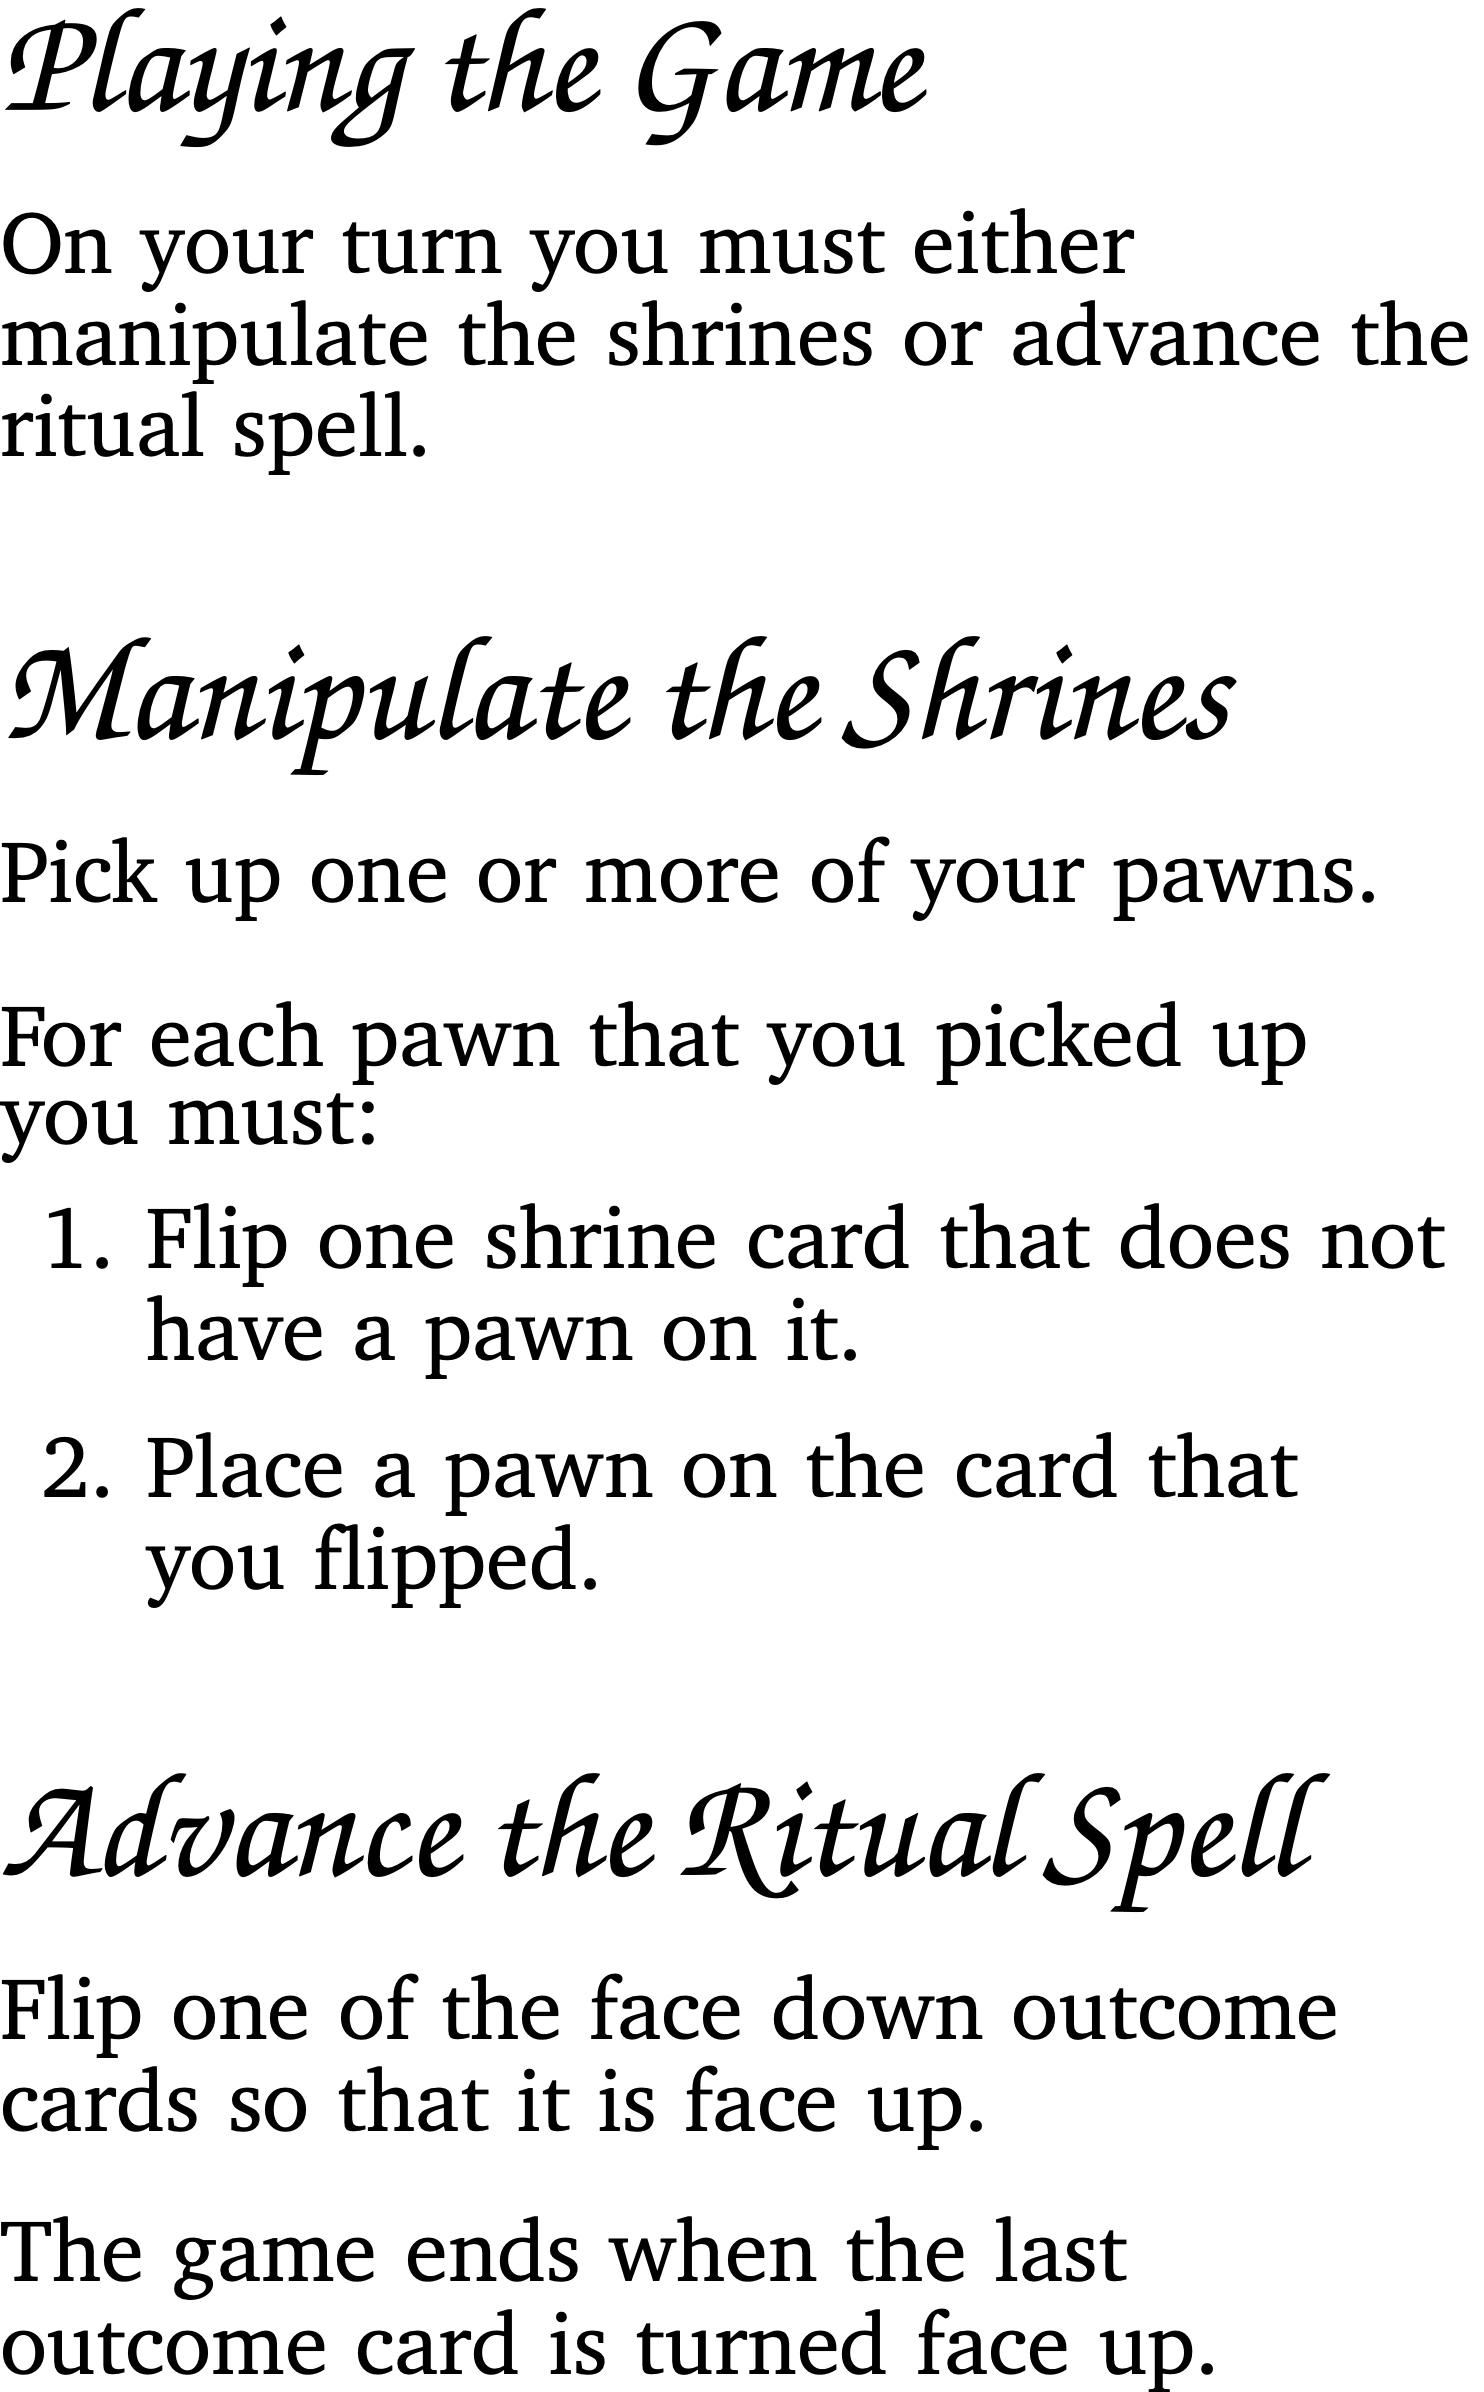
\includegraphics[scale=0.12]{player_aid_turn_text.png}};
\pic[scale=1.5, transform shape] () at (0, 0) {cutguide={Orange}};
\pic[scale=1.5, transform shape] () at (1.5\horizdist, 0) {player_aid_turns={eaglered}};
\node at (1.5\horizdist,0) {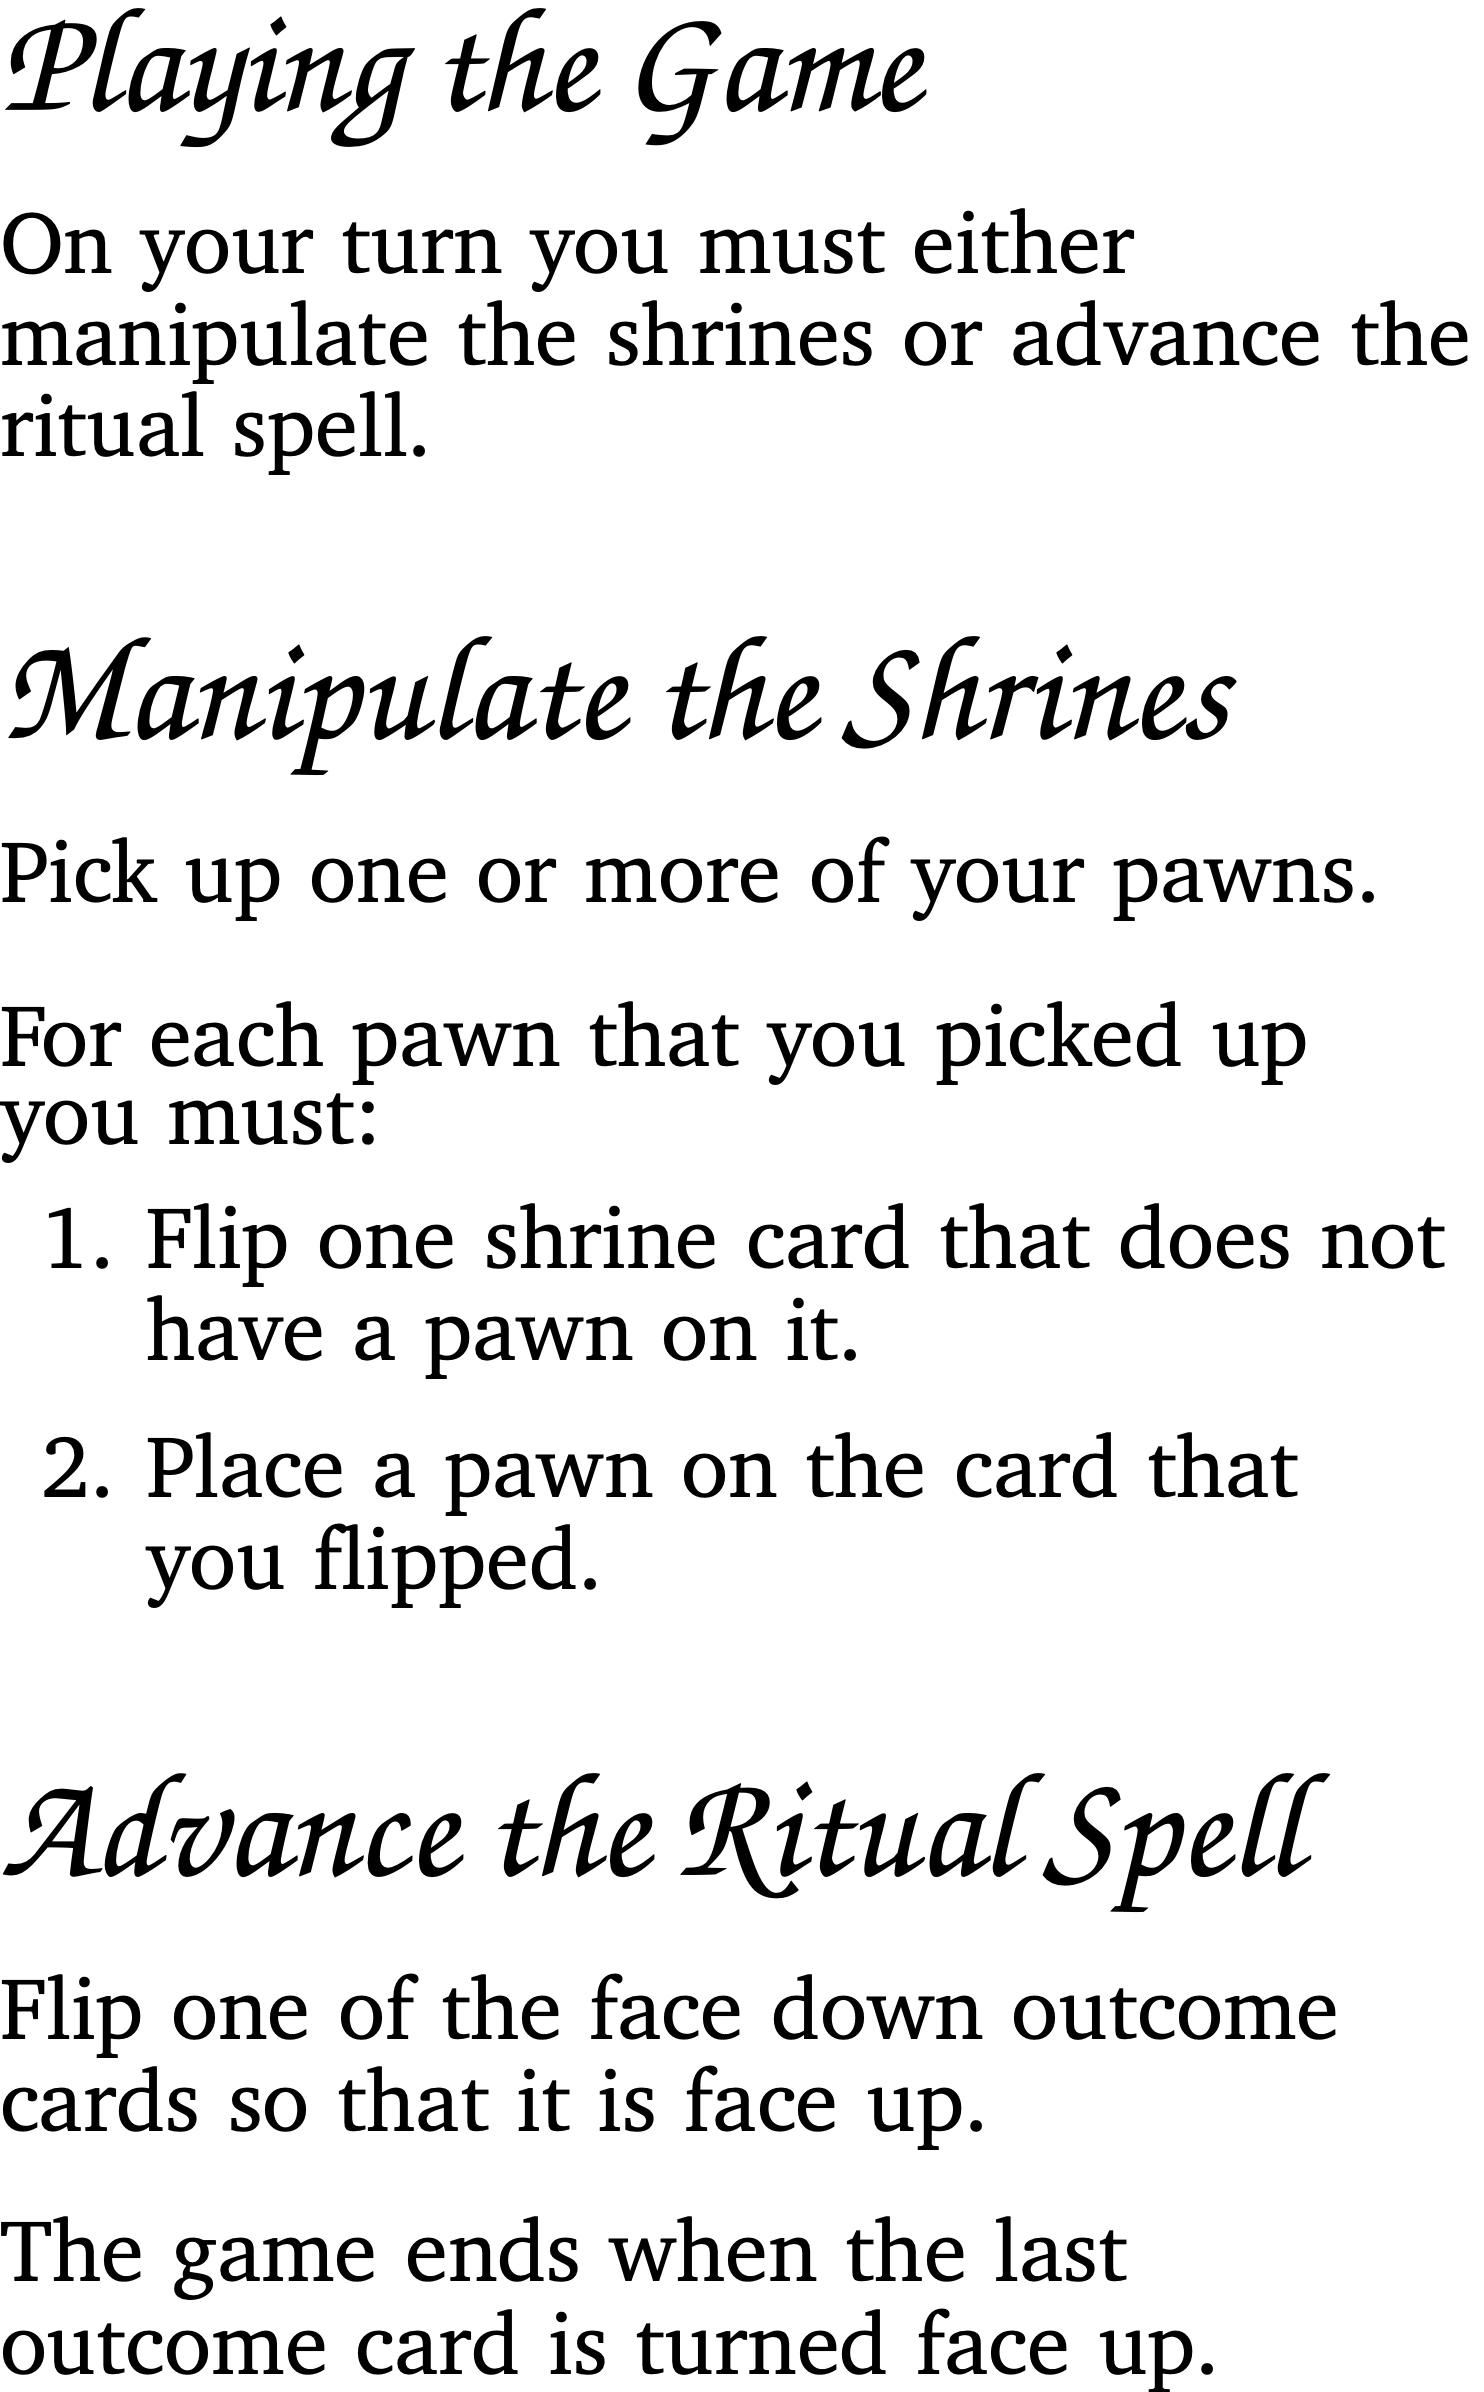
\includegraphics[scale=0.12]{player_aid_turn_text.png}};
\pic[scale=1.5, transform shape] () at (1.5\horizdist, 0) {cutguide={eaglered}};

%\pic () at (0,-\vertdist) {player_aid_turns={hydrapurple}};
%\pic () at (0,-\vertdist) {cutguide={hydrapurple}};
\pic[scale=1.5, transform shape] () at (0, -1.5\vertdist) {player_aid_turns={wolfblue}};
\node at (0,-1.5\vertdist) {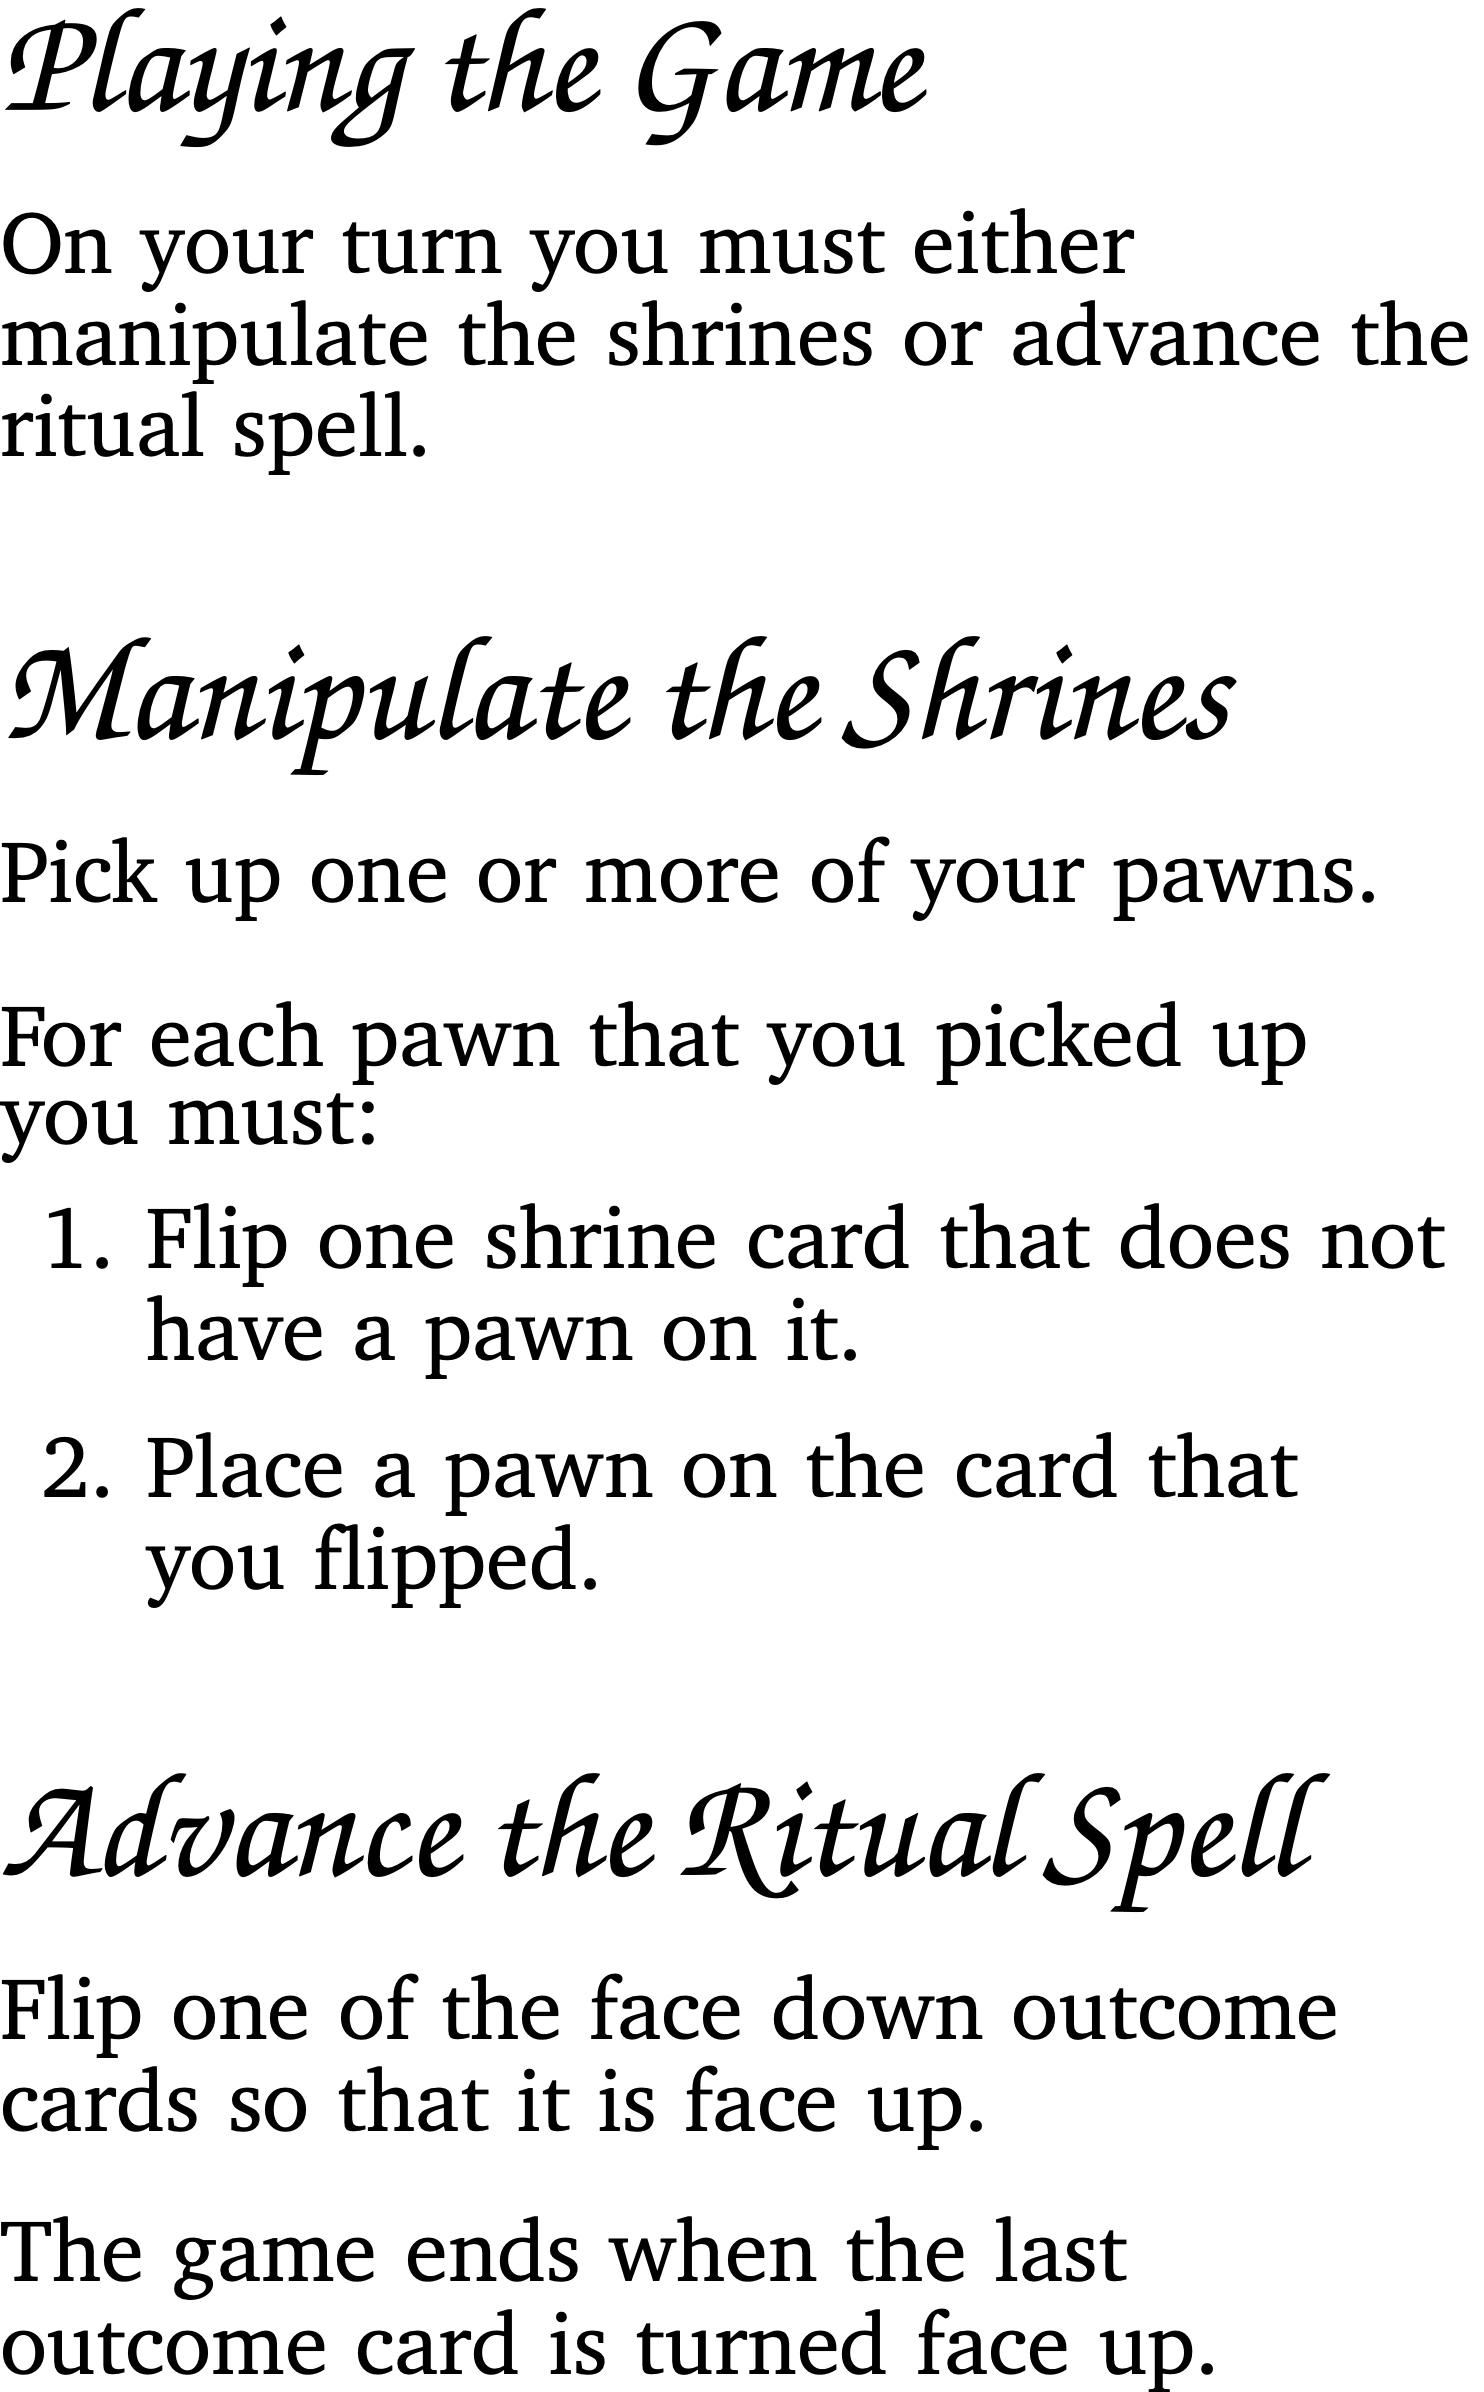
\includegraphics[scale=0.12]{player_aid_turn_text.png}};
\pic[scale=1.5, transform shape] () at (0, -1.5\vertdist) {cutguide={wolfblue}};
\pic[scale=1.5, transform shape] () at (1.5\horizdist, -1.5\vertdist) {player_aid_turns={dragongreen}};
\node at (1.5\horizdist,-1.5\vertdist) {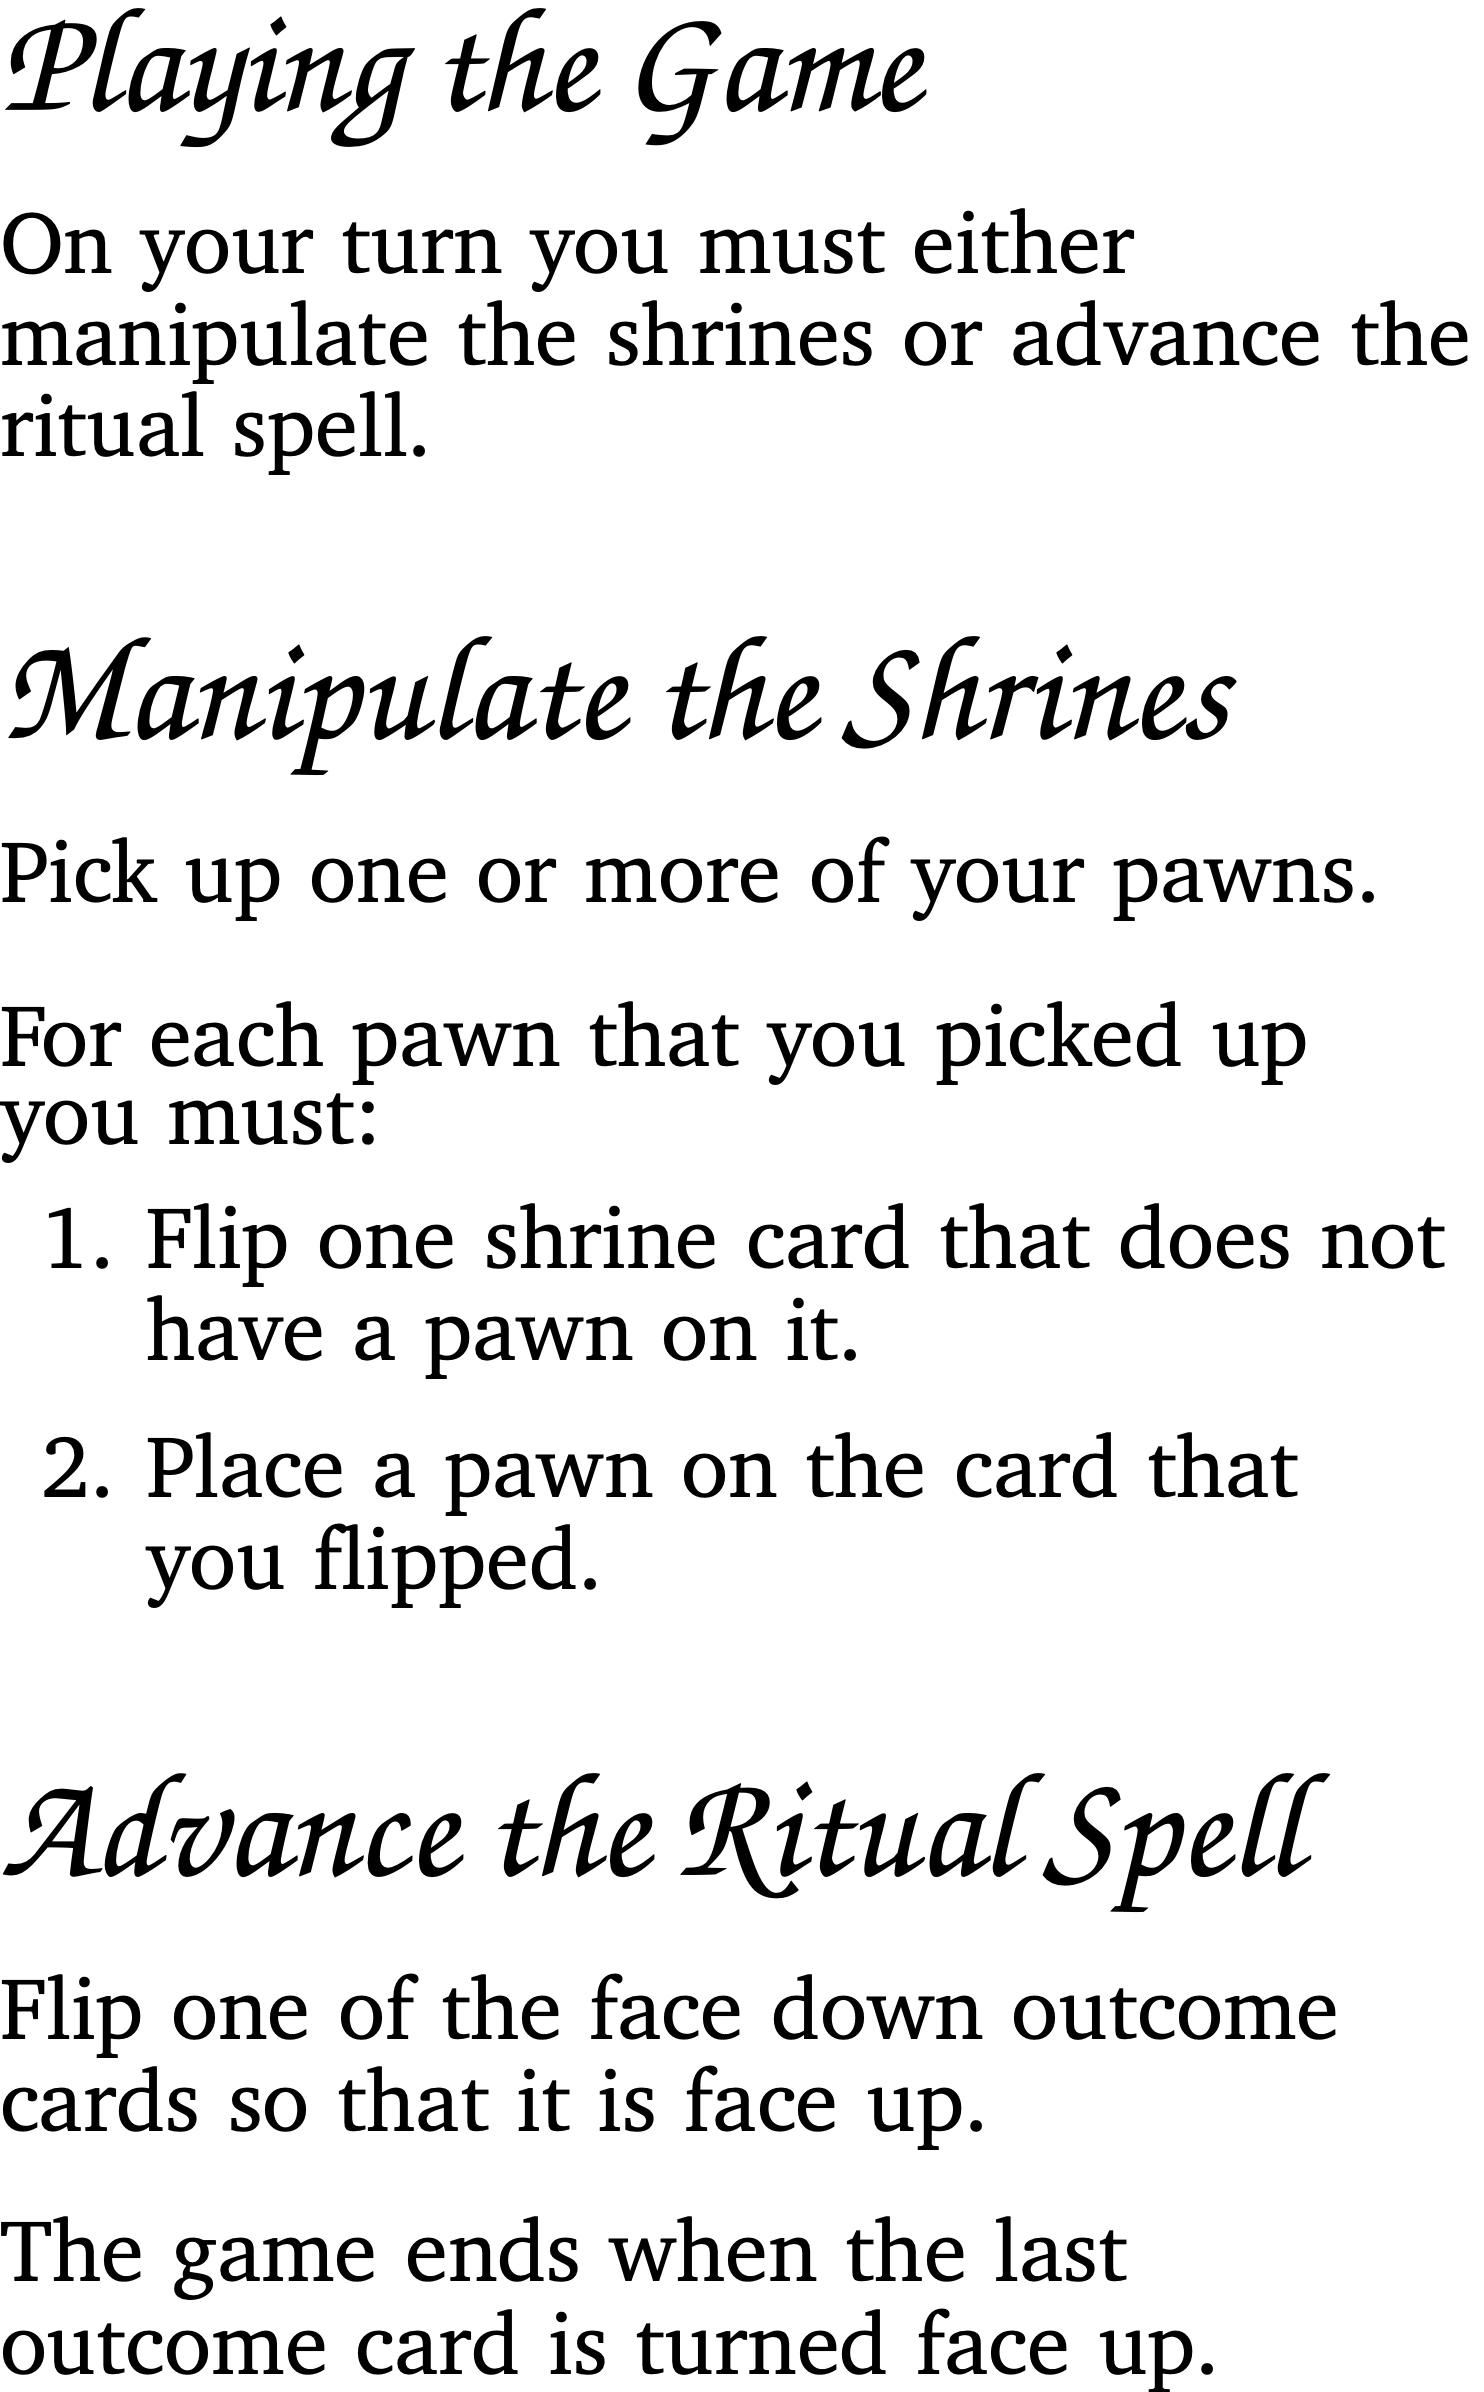
\includegraphics[scale=0.12]{player_aid_turn_text.png}};
\pic[scale=1.5, transform shape] () at (1.5\horizdist, -1.5\vertdist) {cutguide={dragongreen}};
\end{tikzpicture}
\end{center}
\newpage
\setmainfont[Scale=1.0]{TeX Gyre Chorus}\phantom{a}%\setmainfont[Scale=3.0]{TeX Gyre Chorus}
\begin{center}
\begin{tikzpicture}[x=1in, y=1in, transform shape]
\pic[scale=1.5, transform shape] () at (0,0) {player_aid_scoring={kidagold}};
\node at (0,0) {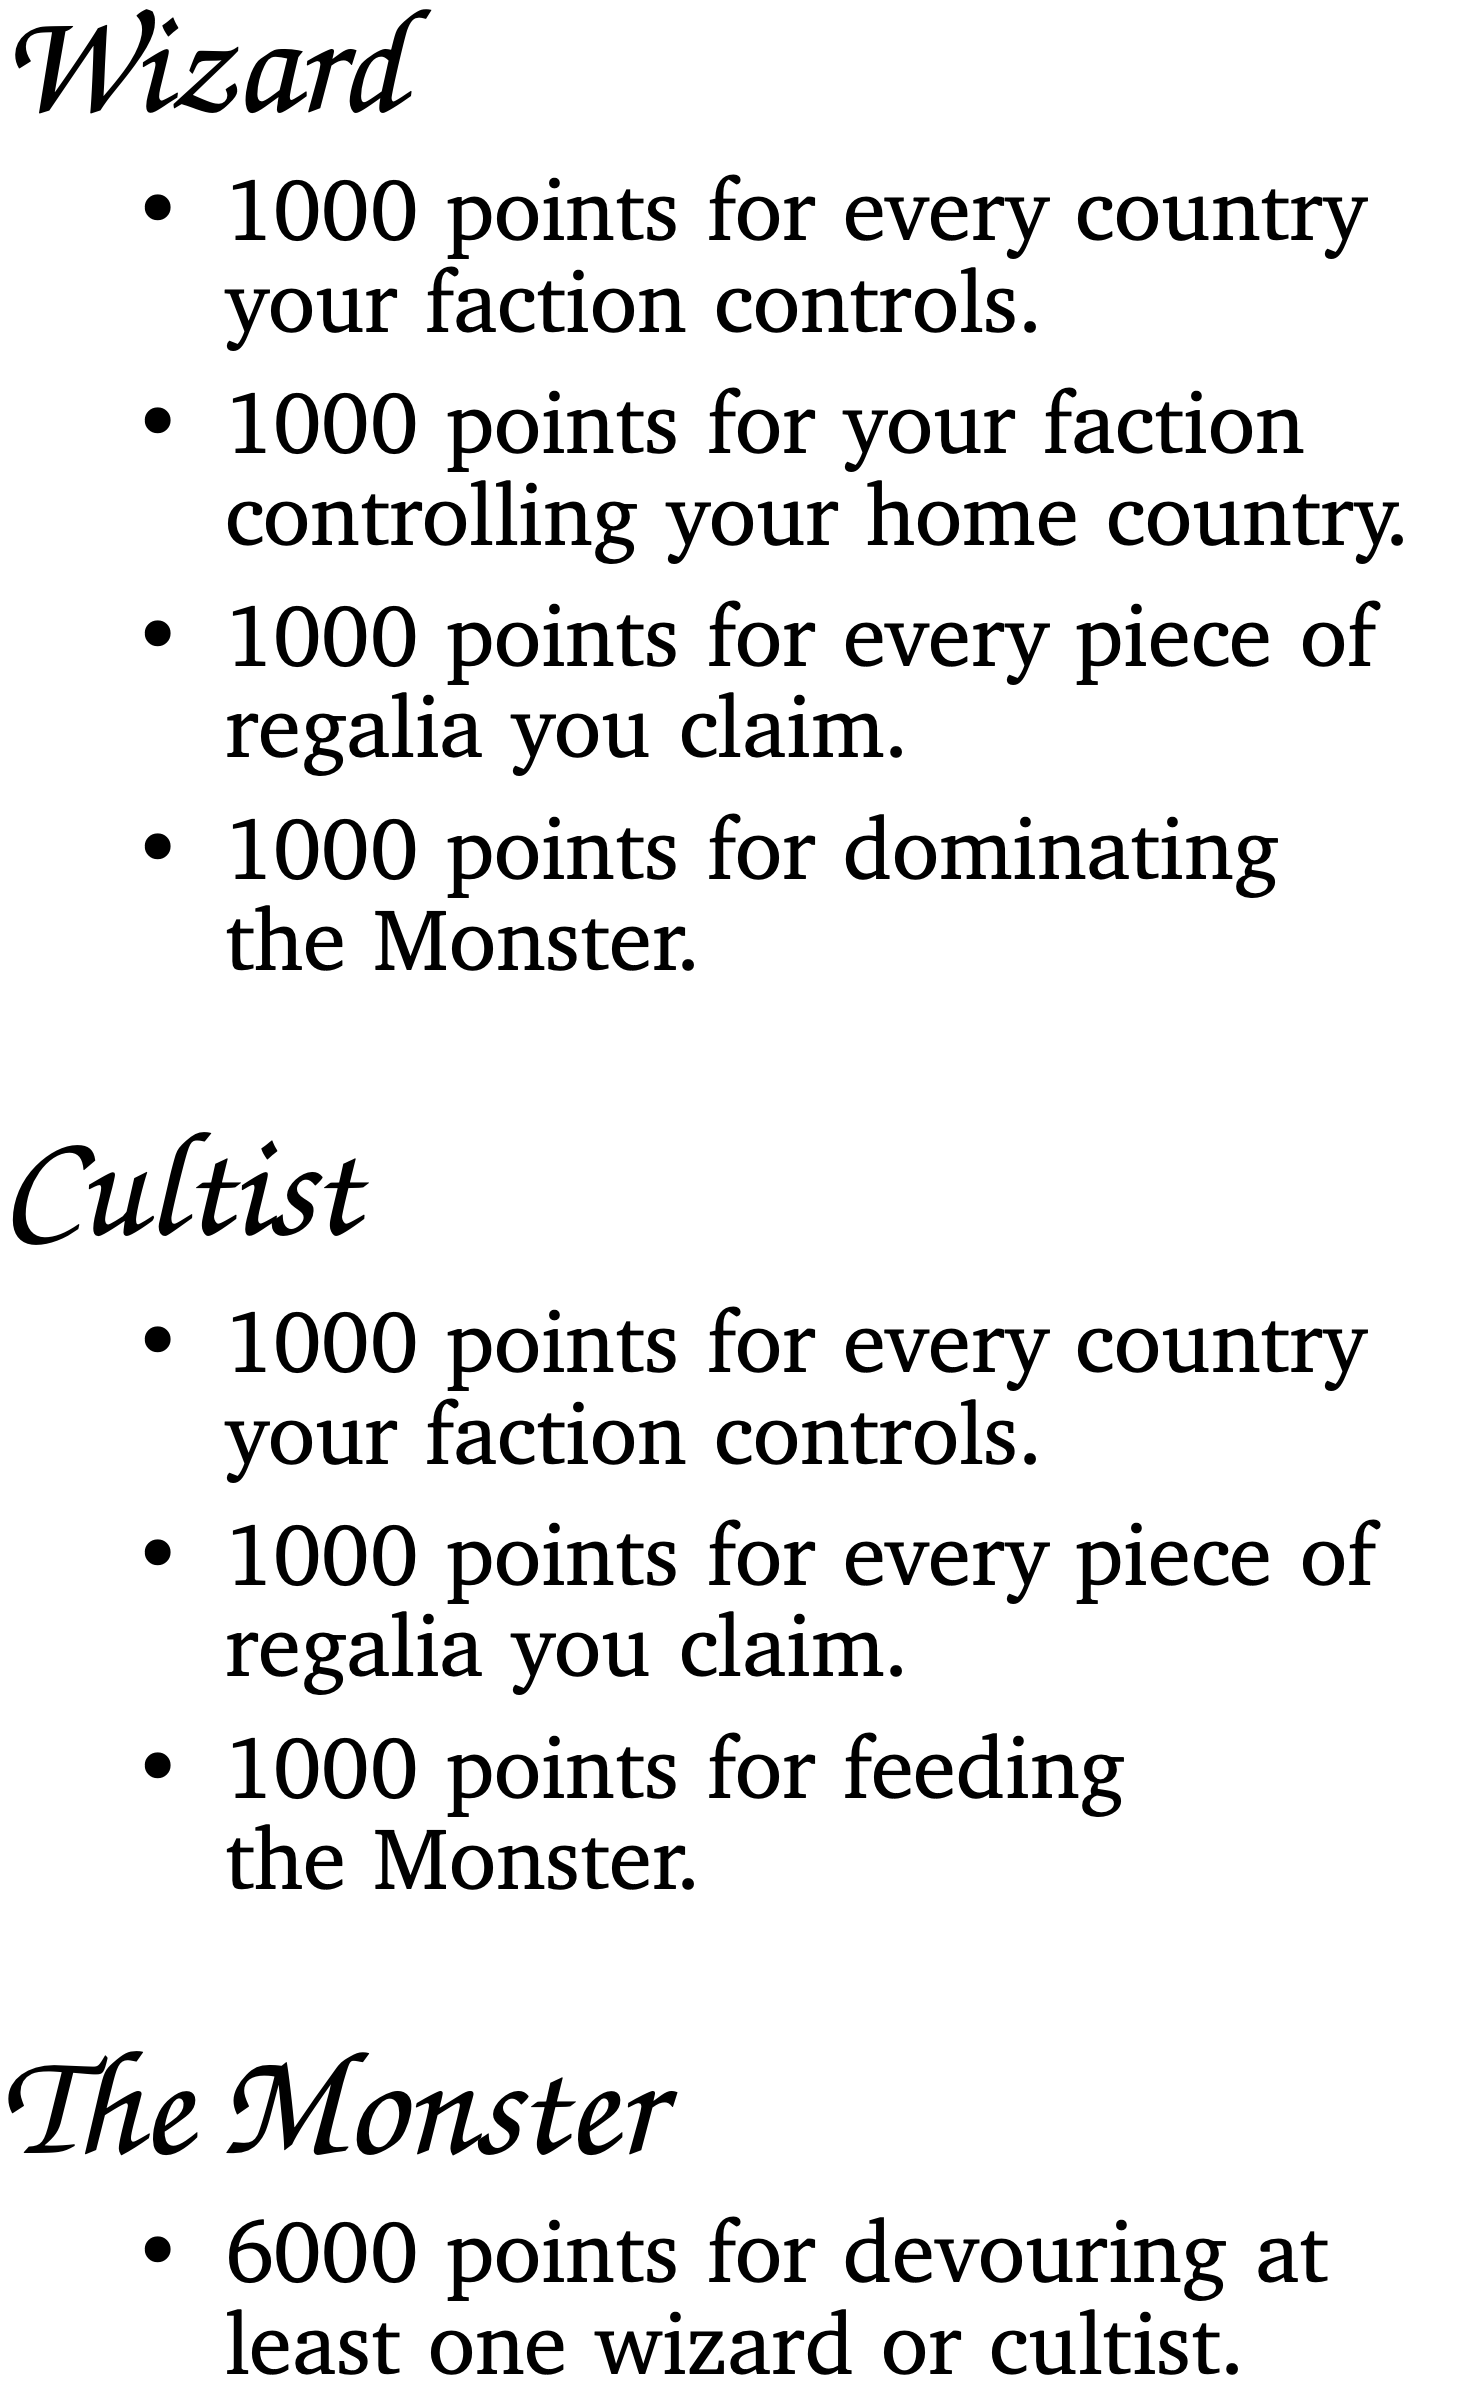
\includegraphics[scale=0.12]{player_aid_scoring_text.png}};
\pic[scale=1.5, transform shape] () at (0,0) {cutguide={black}};
\pic[scale=1.5, transform shape] () at (1.5\horizdist,0) {player_aid_scoring={hydrapurple}};
\node at (1.5\horizdist,0) {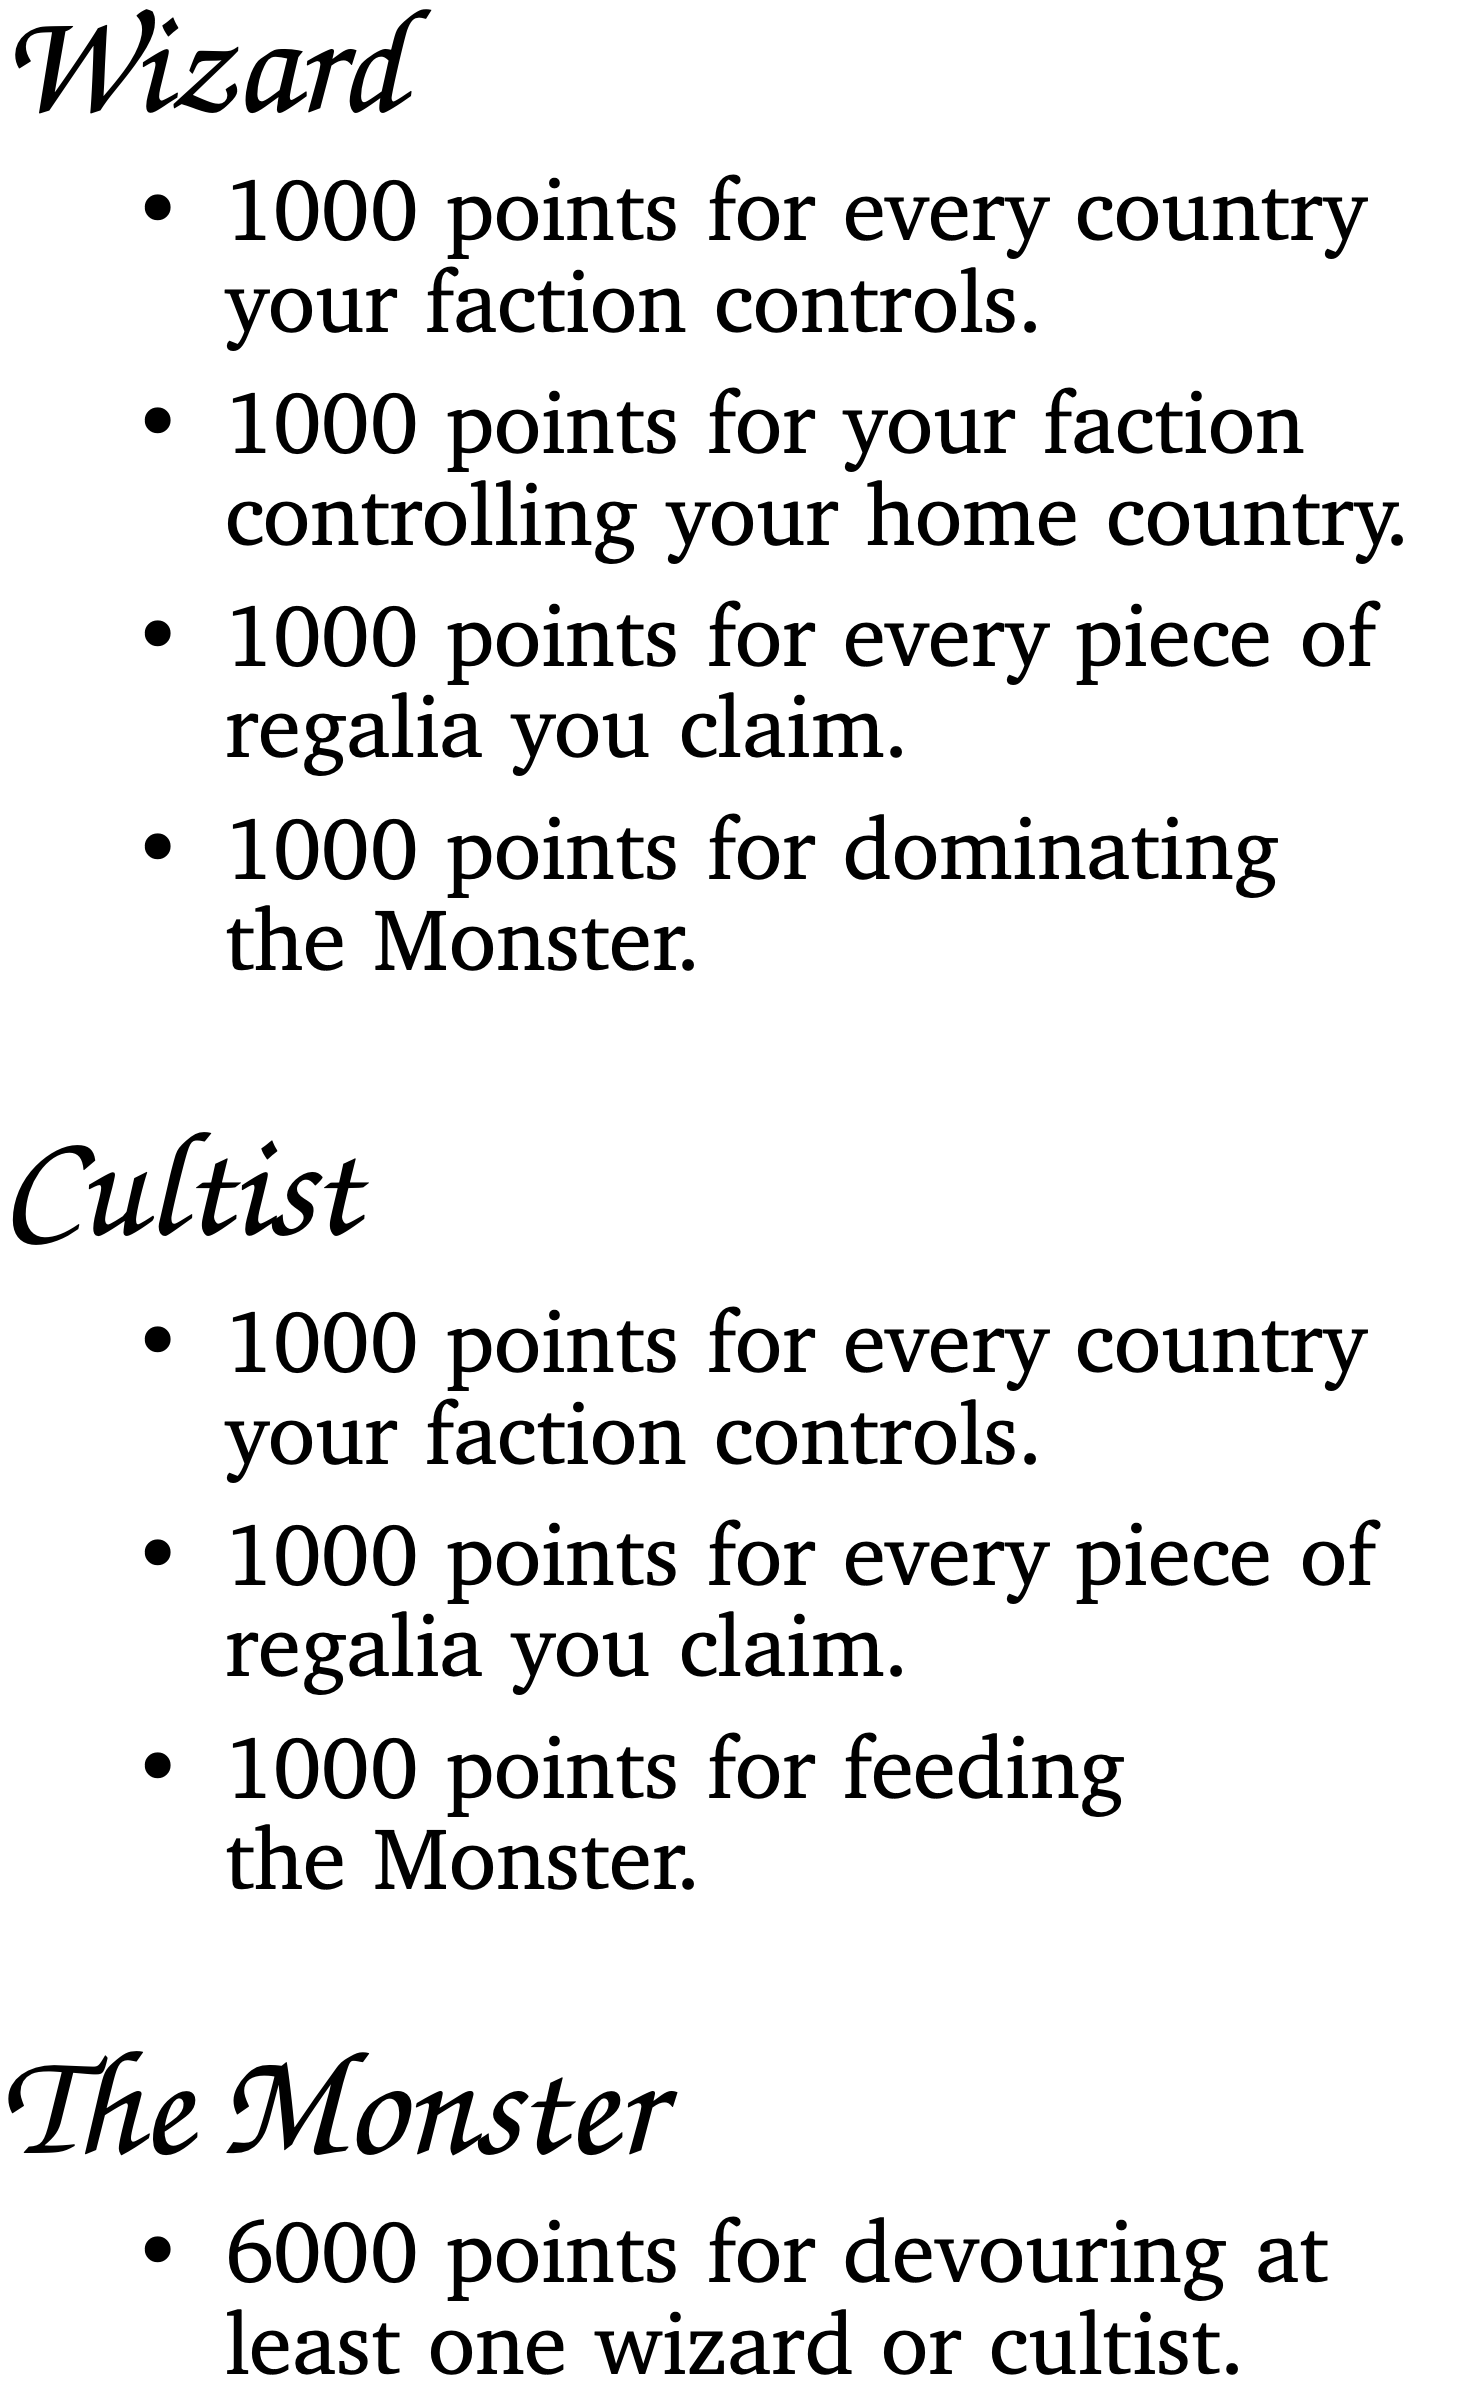
\includegraphics[scale=0.12]{player_aid_scoring_text.png}};
\pic[scale=1.5, transform shape] () at (1.5\horizdist,0) {cutguide={black}};
\end{tikzpicture}
\end{center}
\newpage
\setmainfont[Scale=1.0]{TeX Gyre Chorus}\phantom{a}%\setmainfont[Scale=3.0]{TeX Gyre Chorus}
\begin{center}
\begin{tikzpicture}[x=1in, y=1in, transform shape]
\pic[scale=1.5, transform shape] () at (0, 0) {player_aid_turns={hydrapurple}};
\node at (0,0) {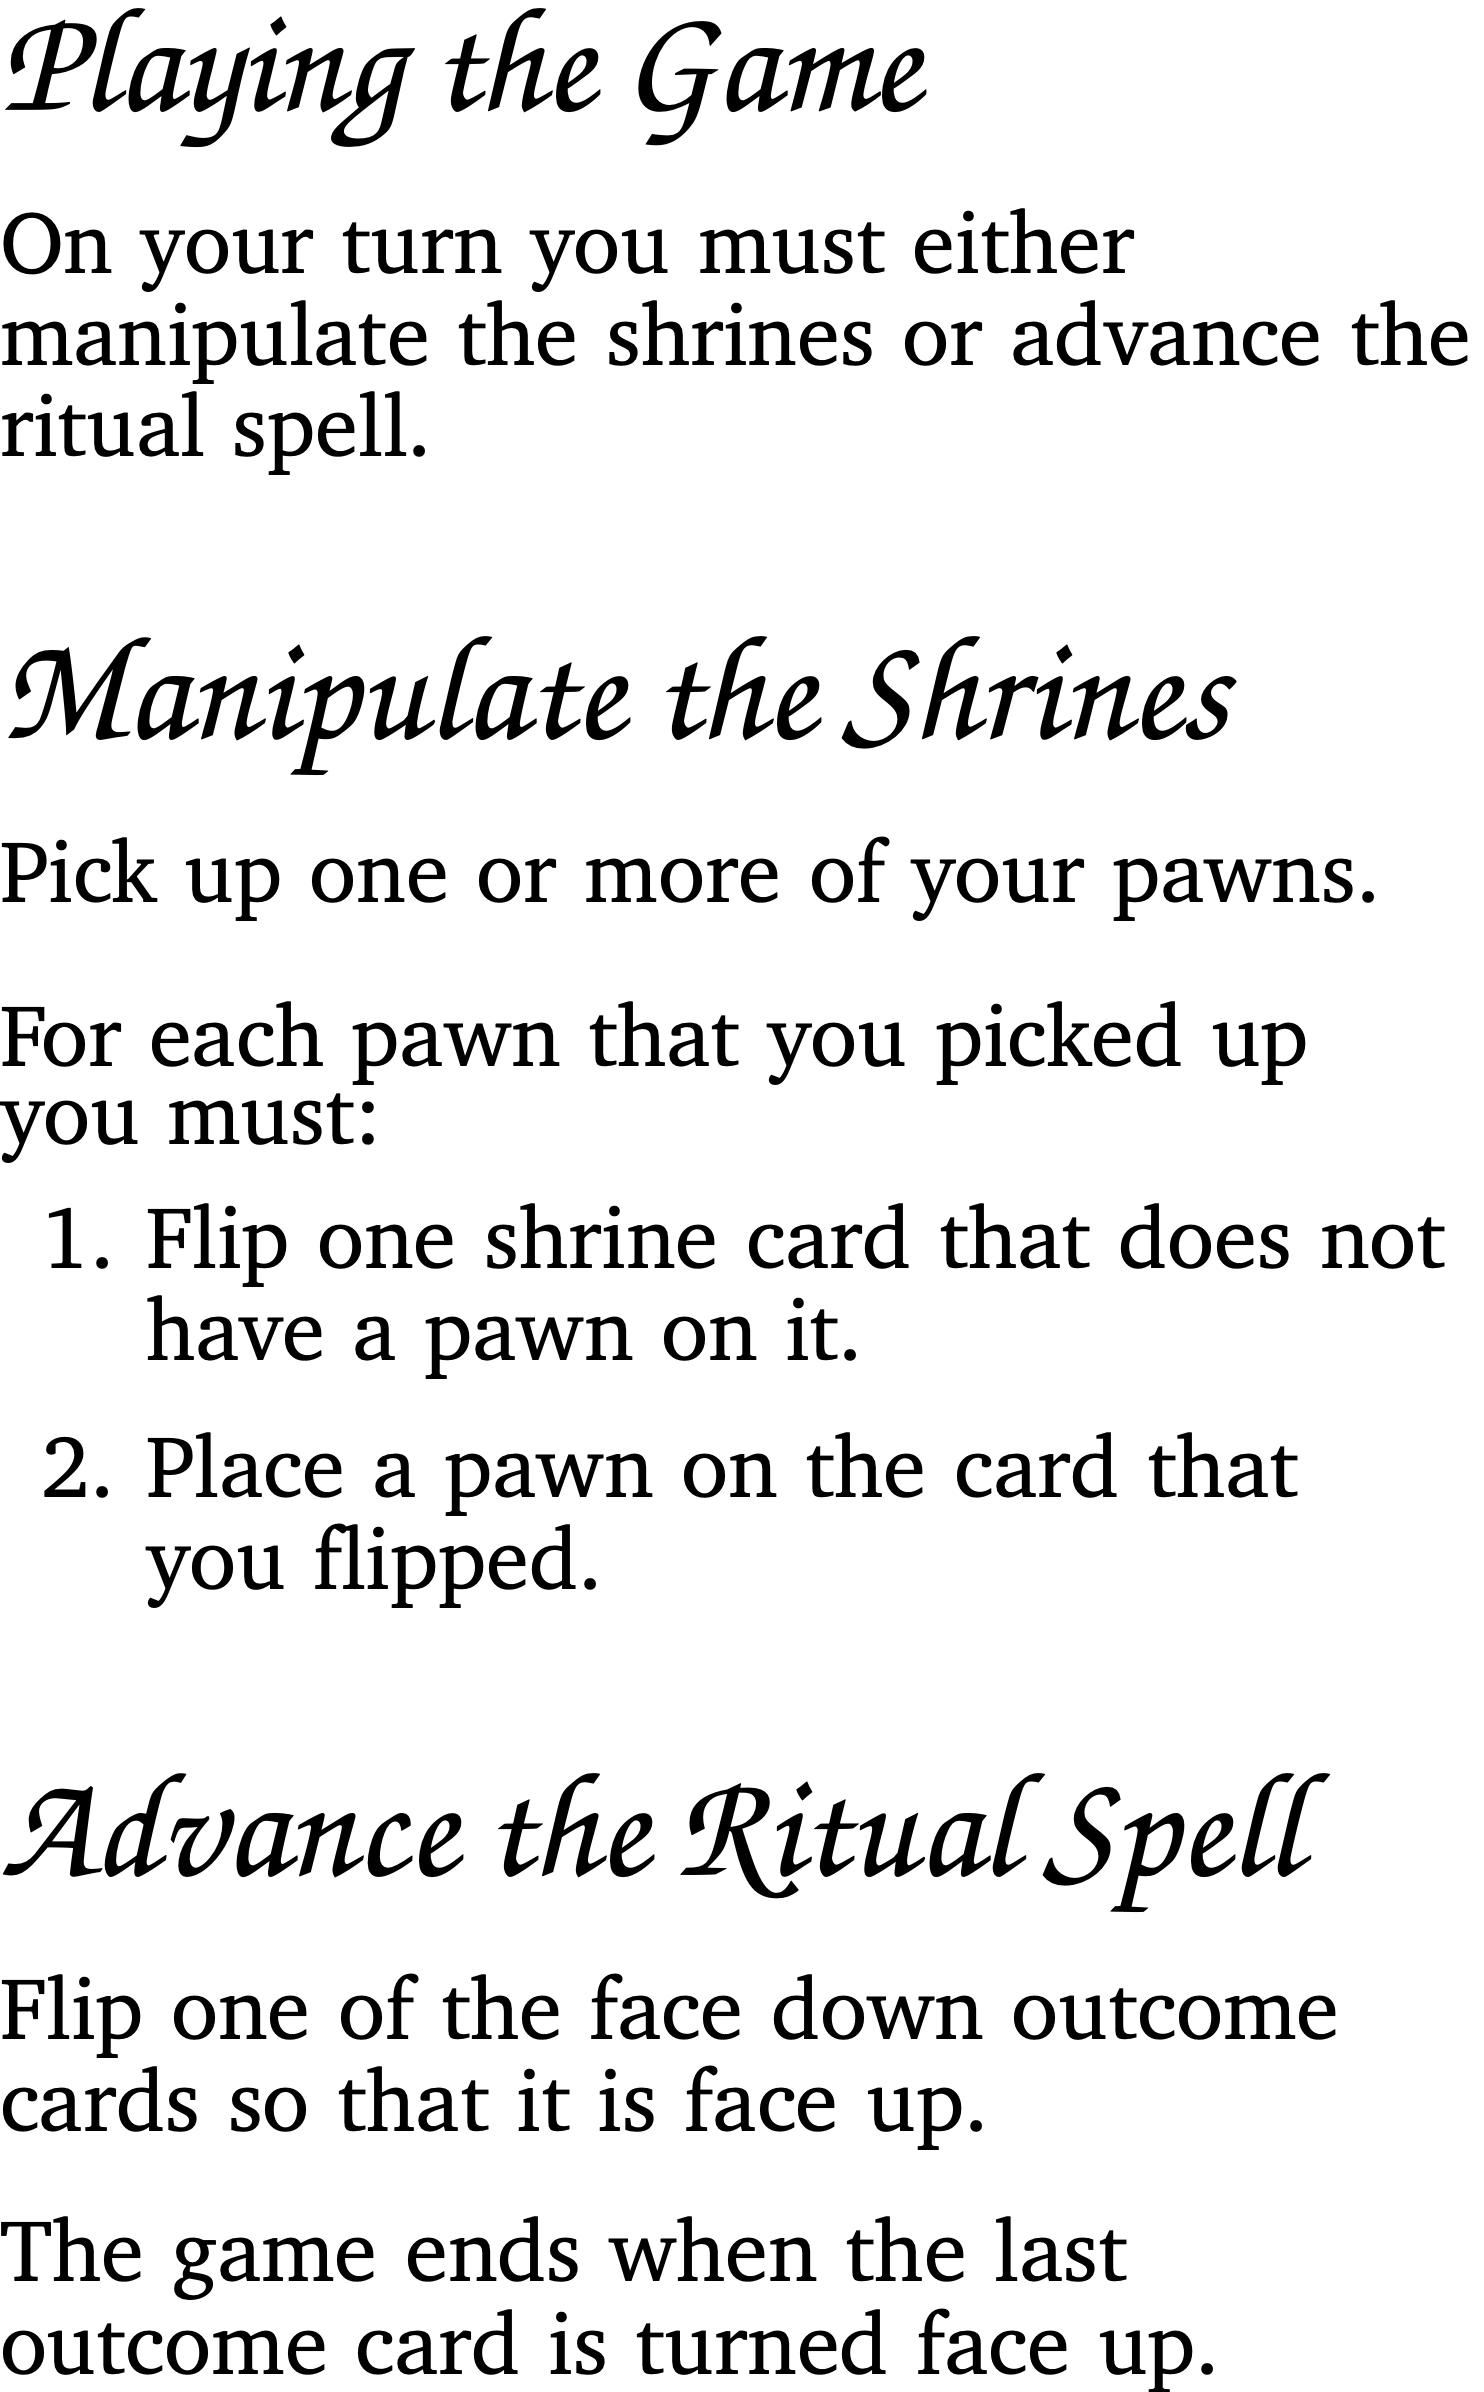
\includegraphics[scale=0.12]{player_aid_turn_text.png}};
\pic[scale=1.5, transform shape] () at (0, 0) {cutguide={hydrapurple}};
\pic[scale=1.5, transform shape] () at (1.5\horizdist, 0) {player_aid_turns={kidagold}};
\node at (1.5\horizdist,0) {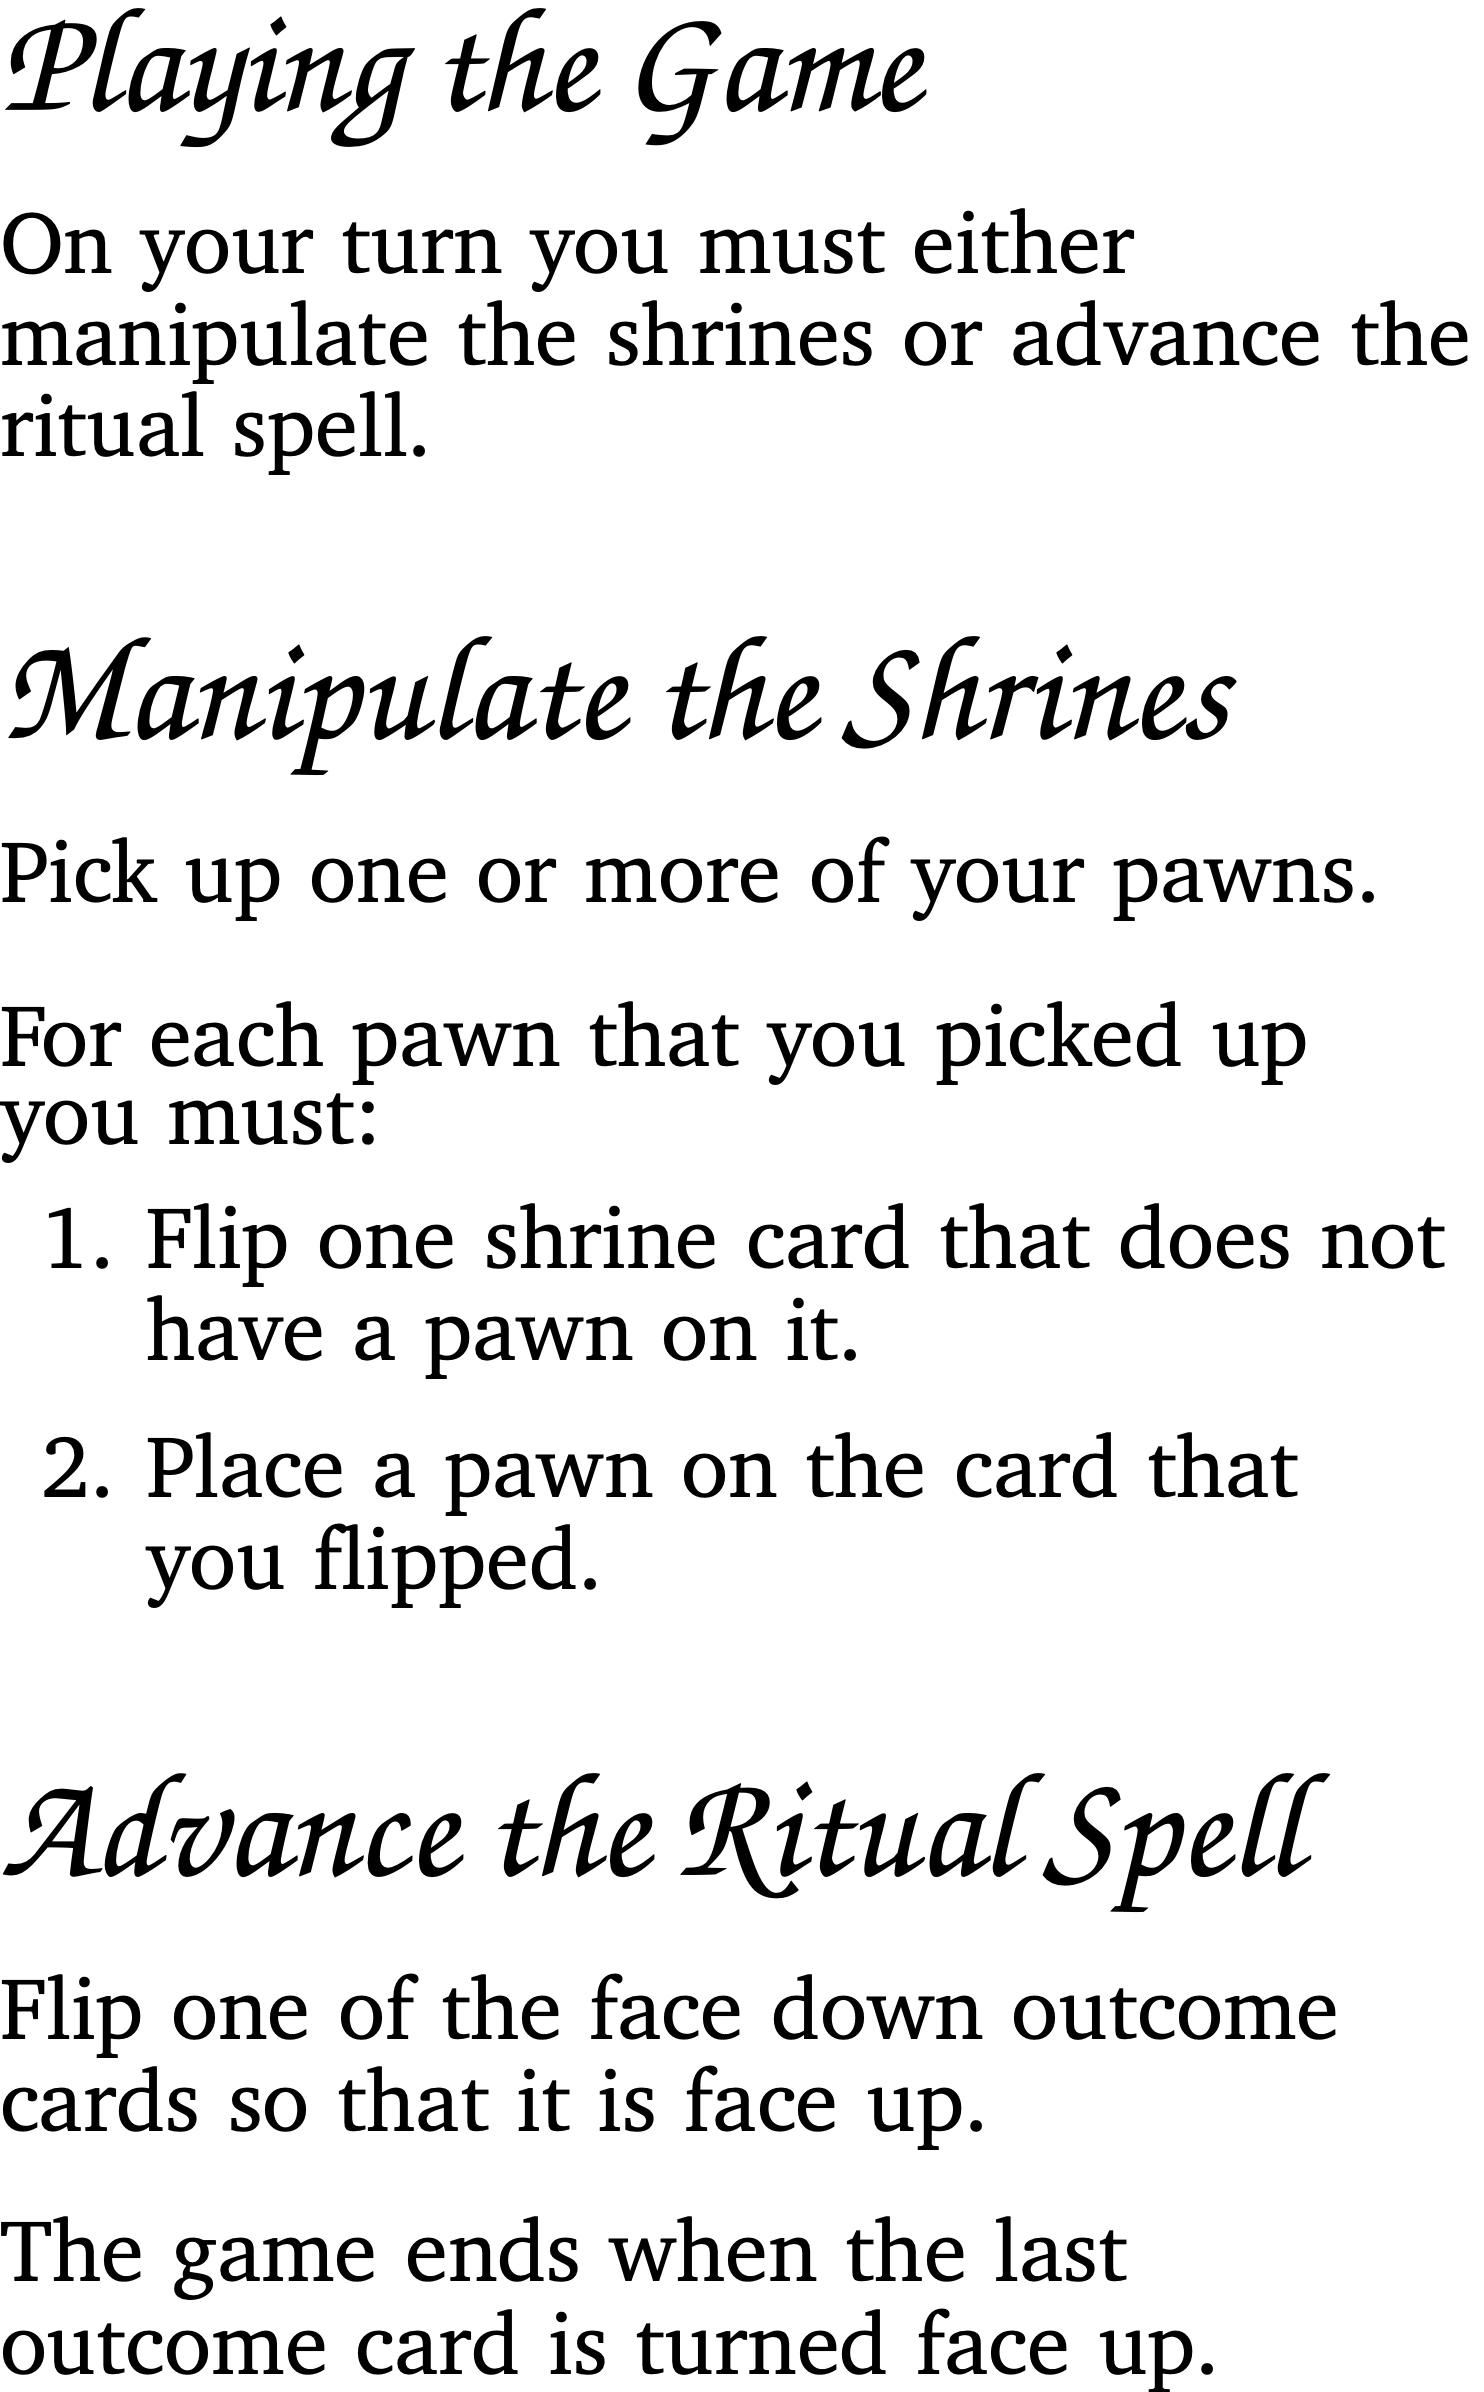
\includegraphics[scale=0.12]{player_aid_turn_text.png}};
\pic[scale=1.5, transform shape] () at (1.5\horizdist, 0) {cutguide={kidagold}};
\end{tikzpicture}
\end{center}

\end{document}